
\newcommand{\CORC}{\mbox{\sf CORC}\xspace}
\newcommand{\EGT}{\mbox{\sf EGT}\xspace}
\newcommand{\tabincell}[2]{\begin{tabular}{@{}#1@{}}#2\end{tabular}} 

\chapter{动态路网中的交通拥堵缓解：面向行程请求流的持续最优路线组合}

\section{引言}

\section{研究背景及应用场景}
    随着基于位置服务的应用的兴起，路径规划服务已经成为我们生活中不可或缺的一部分。路径规划和行程推荐在近几年引起了学者们的广泛研究\cite{DBLP:journals/networks/DumitrescuB03,DBLP:journals/vldb/SharifzadehKS08,DBLP:journals/pvldb/LevinKSS10,DBLP:conf/mdm/ShangLPX13,DBLP:journals/tkde/LiYM13,DBLP:conf/ijcai/ZengCCQCX15,DBLP:conf/wise/XuCYSZZL17}。这些研究的研究目标是基于当前的交通状态为单行程制定最优的路线。值得关注的是，在路径规划服务使用越来越频繁的情况下，大量的用户很有可能会在极短的时间间隔内密集地发布行程请求，特别是在通勤时间等高峰时期，从而形成了持续的行程请求流。在这种新的场景下，实现针对行程请求流的路径规划这一需求变得更加迫切。已经存在的相关研究旨在为行程请求中的单个行程依次制定个人最优路线\cite{DBLP:conf/icde/MalviyaMB11,DBLP:conf/dasfaa/XuGDSL12}。然而，在为行程请求流规划路线时，仅仅基于当前的交通状态以个人最优为最终目标规划个人最优的路线，可能会导致交通拥堵。更合理的路线规划应该考虑到之前已经规划的行程会对未来的交通状态产生影响，因为它们会增加路网中各路段的车流量。
    


    \begin{figure}[tbh]
		\centering
		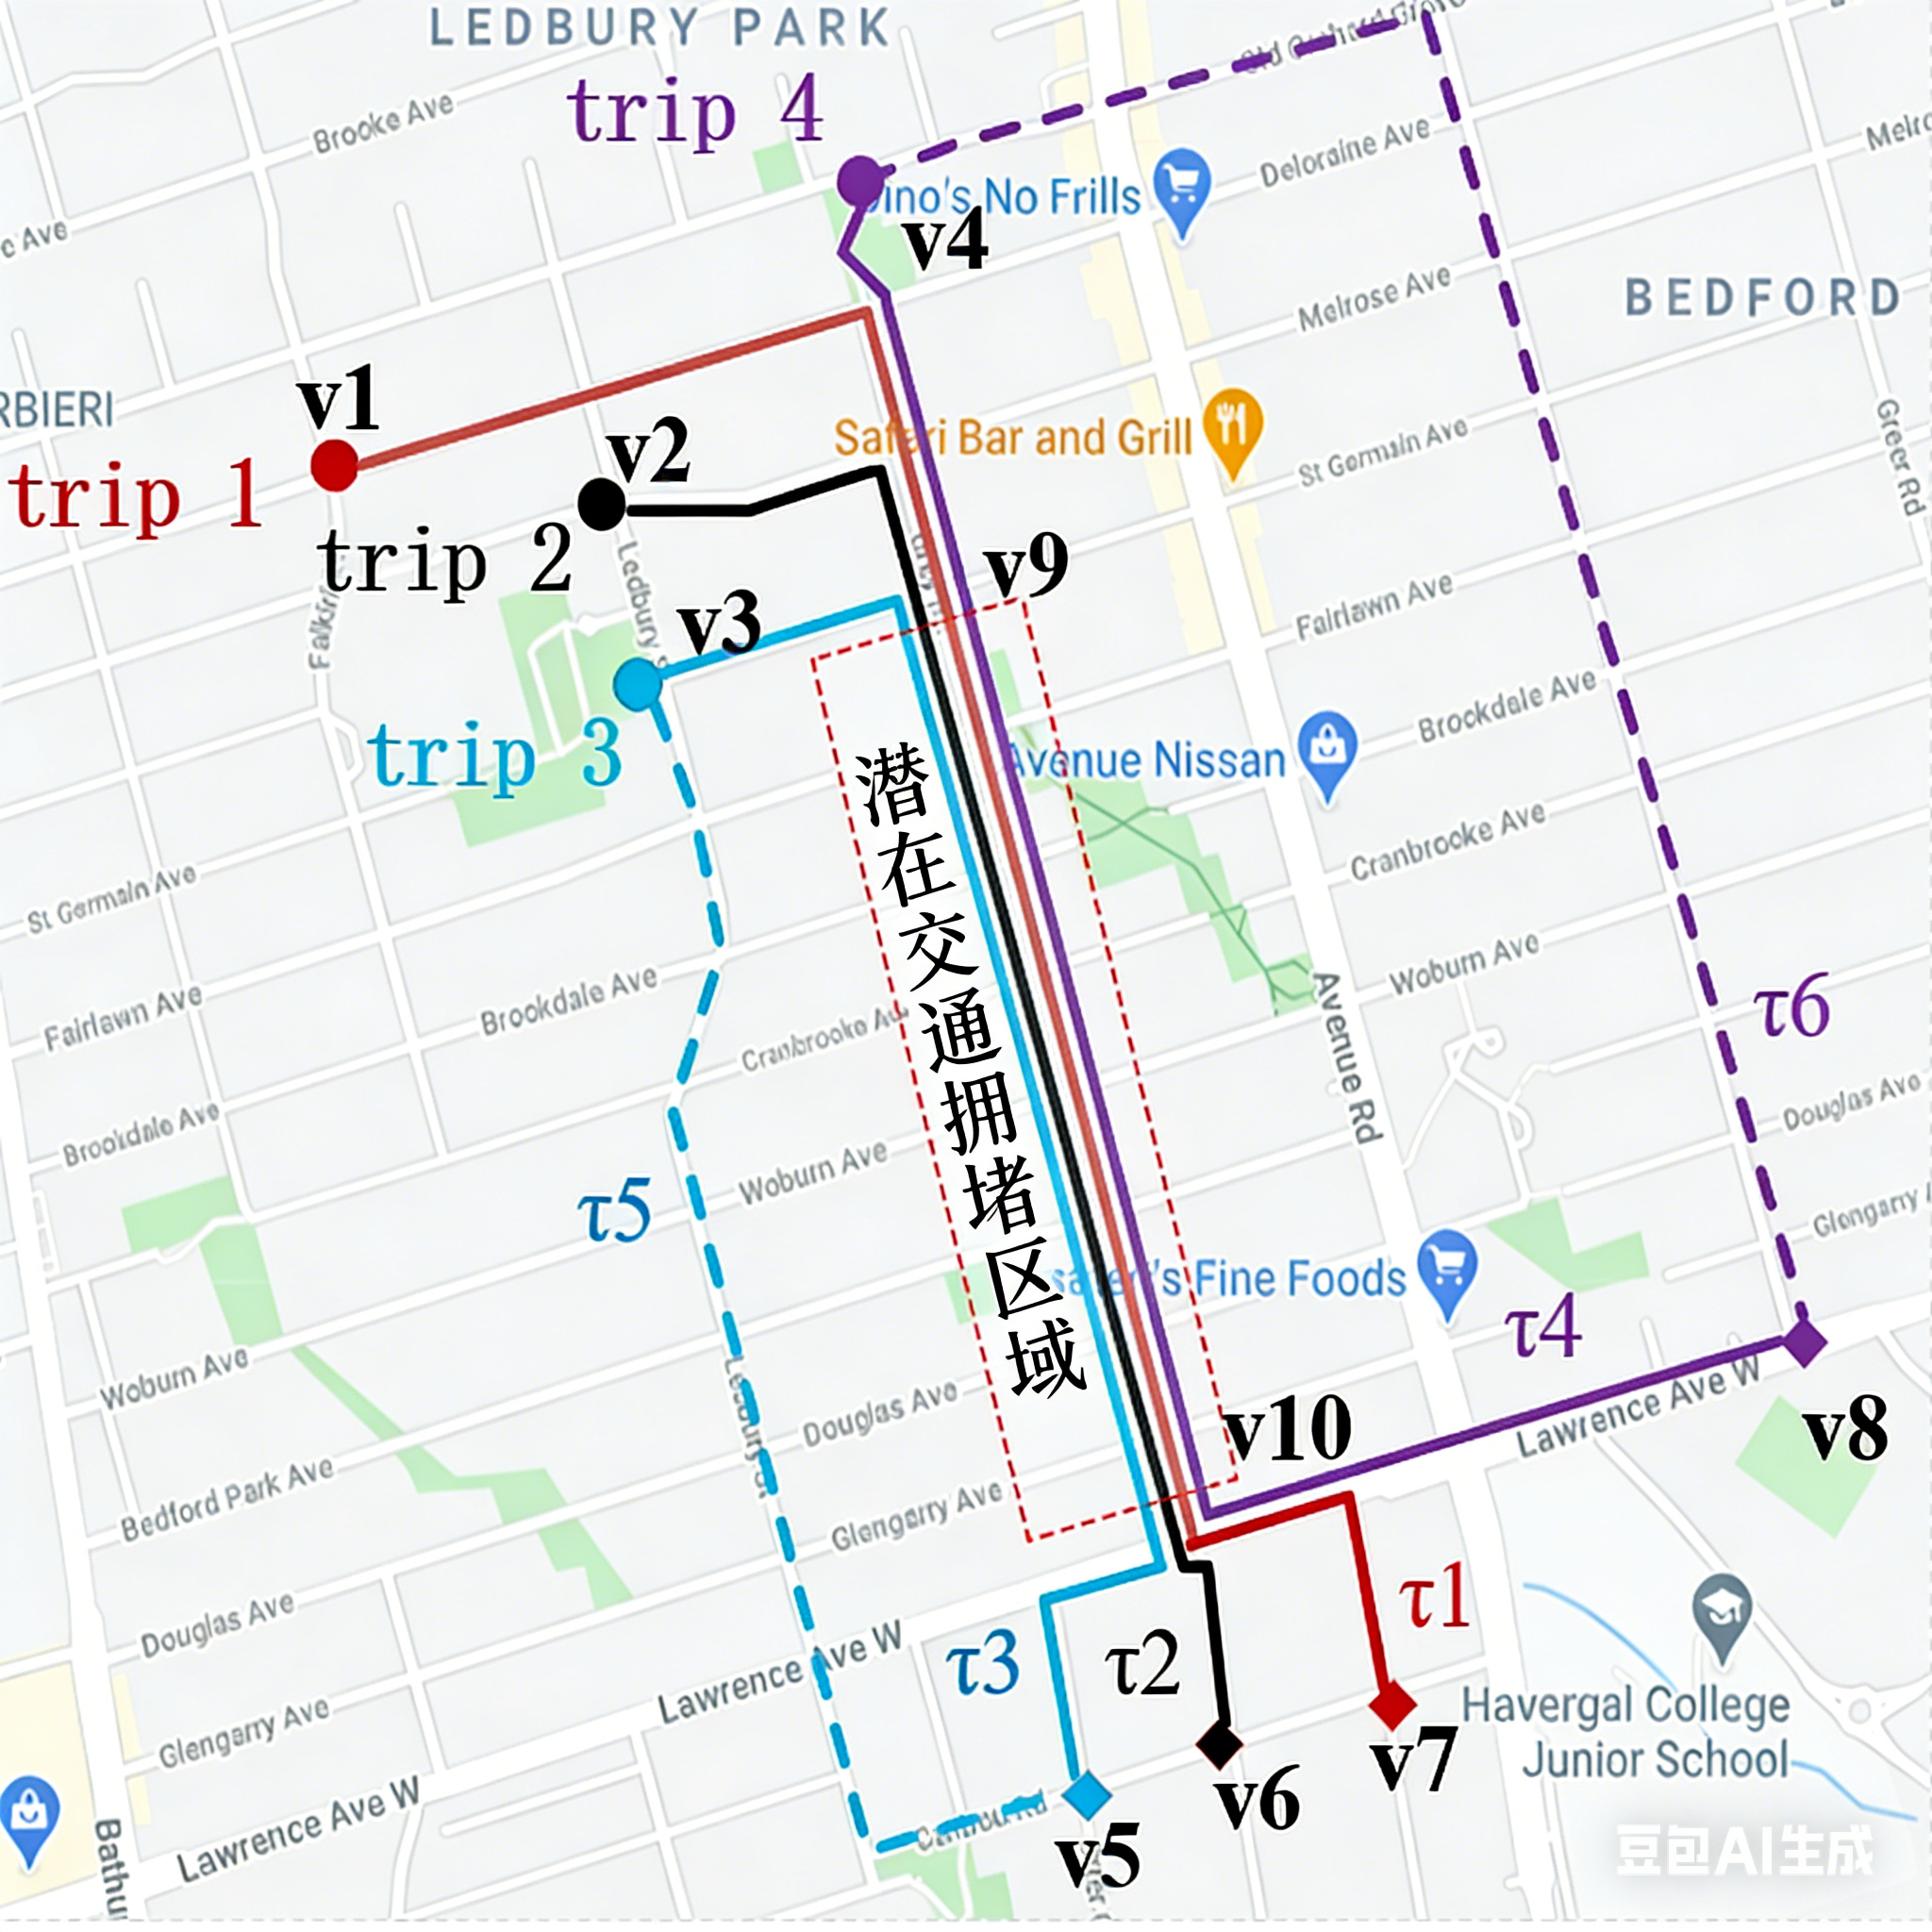
\includegraphics[width=0.6\linewidth]{fig/section3/ex1.png}
		\caption{行程请求和路线}
		\label{fig1:selfaware_ex}
    \end{figure}

以图1为例，图中的每个行程包含一个起点和终点，分别用圆圈和钻石形状标记。顶点$v_1-v_4$是行程1--4对应的起点，而顶点$v_5-v_8$是行程1--4对应的终点。行程请求1--3分别发布于8:00:01,8:00:01,8:00:05。它们的最优路线分别是$\tau_1$,$\tau_2$和$\tau_3$，在图中我们用实线标记。这三条路线预计分别会在[8:02:00,8:05:00], [8:01:40, 8:04:40],[8:01:30, 8:04:30]行驶在路段$e(v_9,v_{10})$。在[8:02:00, 8:04:30], 它们都会都会行驶在路段$e(v_9,v_{10})$，而这也许会导致交通拥堵，从而延路段$e(v_9,v_{10})$所有正在行驶的其他车辆的通行时间。行程4发布于8：00：20，基于在8：00：20这一时刻的交通状态我们为它制定的最优路线为$\tau_4$。很明显，该规划没有意识到路段$e(v_9,v_{10})$由于
之前规划的路线$\{\tau_1,\tau_2,\tau_3\}$，在未来可能会产生潜在的交通拥堵。糟糕的是，我们为行程4制定了最优路线$\tau_4$，该路线再一次经过了路段$e(v_9,v_{10})$，也许会进一步加剧交通拥堵。
综上，给定一组密集发布的行程请求流，为了缓解交通拥堵，我们需要把它们看作一个整体进行路线规划。如例1，我们可以先把行程1--3看作一个整体，考虑到可能产生的交通拥堵。我们可以调整行程3的最优路线为$\tau_5$, 在图\ref{fig1:selfaware_ex}中用虚线表示。对当前到达的行程4，通过把行程1--4看作一个整体，同理我们可以调整其最优路线为$\tau_6$。这些调整后的路线对单个请求来说也许是次优的路线，但路段$e(v_9,v_{10})$的交通拥堵却可以得到大大缓解，行程1--4总的通行时间也会大大减少。通过采用$\{tau_1,tau_2,tau_5,tau_6\}$这一路线组合，行程1--4的总的通行时间可能会是最小的，我们称这样的一个路线组合是最优的路线组合。


\subsection{研究内容与挑战}
本文提出和研究了一种针对持续的行程请求流的路线规划问题：在一个动态路网上给定一组行程请求流，行程请求流中的行程请求数是不断增加的，我们需要找到一个路线组合$\Pi=\{\pi_1,\pi_2,\ldots\}$使得所有在$\Pi$中的路线的总的通行时间最小。其中，每一条路线$\pi_i \in \Pi$是为每一个具体的行程请求$q_i$对应规划的。该问题具有十分广泛的应用场景，包括但不限于城市交通流量管理，实时的路线规划以及持续的拥堵预防上。针对该问题的精确算法具有指数级的时间复杂度，因此不能有效地运用到实际的应用场景中。为了解决这个问题，我们提出了一个自感知的批处理算法。对应的实验研究证明了该算法的准确性和高效性。
\subsection{研究成果与贡献}

\section{问题描述}

\subsection{Dijkstra 算法}
\subsection{位置点间的距离计算}
\subsection{问题定义}

\subsection{路网及其构成}
\begin{definition}[动态路网]
    一个动态路网G=(V,E)是由顶点集V和边集E构成的，其中$E\subseteq V\times V$，顶点代表路段的连接点，交叉点；连边则代表具体的路段。每条边$e(v_i,v_j)\in E$连接着两个顶点$v_i$和$v_j$，这里$v_i,v_j \in V $。为了便于描述，我们假定所有行程请求的起点和终点位置都已经被映射到离它们最近的顶点上。针对每个路段$e$, 我们用$C_e$来代表该路段的车容量，用$T_m(e)$代表在路段$e$的最小通行时间（e.g.，当路段$e$上没有其他车辆时的通行时间）。在我们的设定中，每一个路段的权重 (通行时间)是动态变化的。一个路段的最小通行时间是$T_m(e)$，而实际的通行时间是和该路段上的动态车流量成比例的。
\end{definition}

\begin{definition}[通行时间函数]
    车辆在时刻$t$经过路段$e$的通行时间和当前时刻路段$e$上的车流量$f(e,t)$相关。参照已经存在的研究\cite{Lim2012Stochastic,JavaniPath,DBLP:conf/ijcai/LiCS20}，基于当前时刻路段$e$上的车流量，我们使用下式来计算路段$e$在时刻$t$的通行时间，我们用$T(e,t)$表示。
    \begin{equation}\label{eq:tf}
    	    T(e,t)=T_m(e)\times(1+\alpha\times{(\frac{f(e,t)}{C_e})}^\beta)
    \end{equation}
    其中，$C_e$代表路段$e$的车流量，$\alpha$和$\beta$是由路段的不同性质（e.g.,限速，路宽) 等决定的可变参数。我们的解决方案是和这些参数独立的，如何为这些参数设置合适的值并不在我们的研究范围内。由式\ref{eq:tf}我们可以知道，随着车辆数目的动态变化，每条路段的通行时间也会随之发生改变。
\end{definition}

\begin{definition}[路线及其通行时间]
    我们用一个有限的顶点序列$\langle v_0,v_1,\ldots,v_{|\pi|-1}\rangle$来表示一条路线 $\pi$。假定路线$\pi$出发时间为$t_0$，$t_i$是其经过的顶点$v_i$的预计到达时间(i.e., $t_i=t_{i-1}+T(e(v_{i-1},v_i),t_{i-1})$)。结合式\ref{eq:tf}，我们用式$ET(\pi, t_0)$来计算一条路线 $\pi$的预计通行时间，即路线$\pi$中每个路段的预计通行时间之和，我们用$ET(\pi, t_0)$来表示。

    \begin{equation}\label{eq:tpi}
    ET(\pi, t_0)=\sum_{i=0}^{|\pi|-2}T(e(v_{i},v_{i+1}),t_i)
    \end{equation}
    之后我们使用$\pi.v_0$和 $\pi.v_{|\pi|-1}$ 来分别代表一条路线$\pi$对应的第一个顶点(起点)和最后一个顶点(终点)。
\end{definition}

\begin{definition}[行程请求流]
    我们用$q=(s, d, t)$来代表一个行程请求，其中$s$是该行程的起点位置，$d$是该行程的终点位置，而$t$是该行程的出发时间。$Q=\{q_1,\ q_2,\ldots\}$由多个行程请求组成，代表一组行程请求 流(i.e.,$\forall q_i,q_j\in Q, i>j$:  $q_i.t \geq q_j.t$)。需要注意的是，$Q$ 是以流数据的形式到达的行程请求集合并且$Q$是动态更新的。
\end{definition}

\begin{definition}[全局最优路径规划问题]
    在一个动态路网$G=(V,E)$上，给定一组行程请求流$Q=\{q_1,\ q_2,\ldots\}$和时间间隔$T$，持续的最优路线组合问题 (CORC问题) 旨在不断地处理最近到达的一批行程请求$Q_n=\{q_k,q_{k+1},\ldots,q_{|Q|}\}$ ($Q_n \subset Q \wedge q_{|Q|}.t-q_k.t=T$)，找到一个最优的路线组合$\Pi=\{\pi_1,\pi_2,\ldots\}$使得：
      (1) $|Q|=|\Pi|$; 
      (2) $(\forall \pi_i \in \Pi)\;(\pi_i.v_0 = q_i.s \wedge \pi_i.v_{|\pi_i|-1} = q_i.d)$; 
      (3) 在$\Pi$中规划的所有路线的总的通行时间最小，我们用$TT (\Pi)$来表示所有路线的总的通行时间 (参照公式\ref{eq:gt})。
      	\begin{equation}\label{eq:gt}
        TT (\Pi)=\sum_{i=1}^{|\Pi|}ET(\pi_i,q_i.t)
	\end{equation}
\end{definition}


\section{精确遍历算法}
针对CORC问题，一个简单直接的办法就是对每一个行程请求，搜索起点和终点间可能存在的所有路线，然后对所有的路线组合进行遍历评估，比较各个路线组合所有路线总的通行时间，最终筛选出具有最小通行时间的路线组合。具体来说，对于每一个行程请求$q_i\in Q$，我们可以采取深度优先算法(DFS)来查找从起点$s_i$到终点$d_i$可能存在的所有路线。其中，我们可以应用一些剪枝策略来加速深度优先搜索。随后，对于每一个路线组合我们计算它所有路线总的通行时间。最终，我们返回具有最小通行时间的路线组合作为返回结果。
精确算法比较简单直接，便于理解。当行程请求数量|Q|较小时，精确算法可以在有限时间内得到最优解。但是，当行程请求数量|Q|很大时，精确算法显然大量的计算时间，不能运用到实际的应用场景中。



\section{自感知的批处理算法}


为了高效解决CORC问题，我们提出了一个自感知的批处理算法 (SBP算法)，该算法主要包含两大组成部分：(1)初始路线搜索和(2)批优化处理。具体来说，给定一组行程请求流$Q_n$，我们首先采用初始路线搜索生成一个高质量的初始路线组合$\Pi_n$，该组合包含了为该行程请求流中的每个请求指定的初始路线。接下来，我们执行批优化处理对初始路线组合中的每个初始路线进行优化。最终，我们将优化后的路线组合$\Pi_n$加入到全局的路线组合$\Pi$中去。每当我们处理完一批行程请求后，我们返回$\Pi$作为实时的规划结果。我们的自感知思想合理考虑了新规划的路线会影响未来的交通状态这一事实, 即规划的路线会增加一些路段的车流量从而影响该路段的实际通行时间。
\subsection{初始路线搜索}
初始路线搜索的目标是为新一批到达的行程请求流中的每个行程请求规划一条高质量的个人路线。每个路段的动态车流量由两部分组成的，一部分是在我们规划系统中的请求车辆所造成的交通流量，即我们规划的路线在各路段上造成的车流量，我们称之为系统内的车流量，一部分是系统外的车流量即在各路段上没有使用我们规划系统的车辆数目，我们把系统外的车流量直接作为算法输入。
\subsubsection{路段标签}

为了实现对系统内车流量的快速计算，我们在每个路段上维持一系列的路段标签$L_e=\{l_1,l_2,\ldots\}$。这些路段标签记录了经过该路段的路线在该路段的时间信息。每个路段标签$l_i=\{t_a,t_b\}$记录了一条特定的路线进入路段$e$的时间$t_a$以及离开该路段的时间$t_b$。刚开始没有行程请求的时候，每个路段维持的路段标签是一个空集。之后每当我们处理完一批新的行程请求集合的时候，对应路段的路段标签会进行动态地更新。


	
	
\subsubsection{系统内的车流量计算}
 我们可以快速地计算在各个路段上由我们规划系统规划的路线所产生的车流量。由我们规划系统规划的路线在路段$e$, 时刻$t$所造成的车流量,也就是满足$[l_i.t_a, l_i.t_b] \ni t$的路段标签$l_i$的数量，其中$l_i \in L_e$。在我们的实验中，我们应用了一个优先队列来加速计算。
 

\subsubsection{通行时间下界}
我们用一个启发值$H(v_i,v_j)$来代表从一个顶点$v_i$到另一个顶点$v_j$的通行时间下界。给定最小的系统外的车流量作为静态的车流量输入，该下界是由Dijkstra 算法~\cite{Edsger1959A}预计算的。在本文中，我们将非请求车辆的车流量直接作为算法输入。


 
 
\subsubsection{算法描述}
算法~\ref{alg:alg1}提出了初始路线搜索的伪代码。算法输入包含一个动态路网$G=(V,E)$，一个行程请求$q=(v_s,v_d,t)$，所有两点间的通行时间下界$H(v_i,v_j)$，所有路段的路段标签集合$\mathcal{L}=\{L_{e_1},L_{e_2},...\}$。算法输出为行程请求$q$制定的一条初始路线。每个顶点$v\in V$ 包含以下记录信息: 从起点$v_s$到达该点的精确通行时间$t_s$；从该点到达终点的通行时间下界$t_d$；从起点到达该点的最小时刻$et$以及一个前驱节点记录$pred$。首先，我们初始化每一个顶点$v\in V$的信息记录，设置 路线 $\pi$是一个空集 (line 1)。接着我们把起点$v_s$加入一个优先队列$PQ$中。该优先队列$PQ$内部对顶点对象按照该点的$v.t_s+v.t_d$的值从小到大排序，队头元素为
具有最小$v.t_s+v.t_d$的顶点 (line 2)。在搜索过程中，每一次我们从$ PQ $选出对头元素$ v $并探索它的邻接顶点。具体来说，每一次我们选出的$ v $都具有最小的$v.t_s+v.t_d$，之所以这样选择，是基于这样的顶点扩张可能会产生最小的通行时间 (line 4)。如果选择的$v$是行程请求的终点$v_d$，我们就利用相应节点的前驱节点记录生成一条路线$\pi$，并将$\pi$作为结果返回 (lines 5--11)。如果选择的$v$不是行程请求的终点$v_d$，对于每一个从顶点$v$出发的路段$e$，我们计算当前时刻该路段的车流量 (line 13)。
对于路段$e(v, v')$的结束点$v'$，我们需要检查该点能否通过顶点$v$到达，并且所花的时间比从其他点到达该点更小 (line 14)。如果满足，我们将分别更新顶点$v'$对应的$t_s$, $et$和$pred$
记录 (lines 15--17)。接下来，如果顶点$v'$不在优先队列$PQ$中，我们将其加入。当优先队列$PQ$为空或者我们已经扩张到行程请求对应的终点时，初始路线搜索算法终止。


初始路线搜索： 对于每一个新到达的行程请求（包含起点，终点，出发时刻），寻找一条在出发时刻出发，从起点能最快到达终点的路径（最短路径）。假设车辆通过特定路段的时间是和该路段的属性和车流量决定的，而车流量由两部分组成。一部分是非请求车辆车流量，即没有使用我们路线规划系统的车辆，直接作为输入数据，不是我们研究的范畴；一部分是请求车辆的车流量，即使用了我们规划系统的车辆，这些车辆按照规划的路线行驶而在经过的路段上增加的车流量。由于路网每个路段车流量是动态变化的，通行时间也会随之动态变化，我们就是要在这样一个动态变化的路网中寻找从出发时刻出发，起点到终点的最短路径。

初始路线搜索过程从起点开始，对与起点相连的邻接顶点做网络扩张，接着选择一个新的顶点继续扩张，直到扩张到终点。我们的扩张策略是，每次选择一个最可能最快到达终点的顶点作为下一个扩张顶点，什么是最可能最快到达终点的顶点呢？即 （从起点到该点的精确耗时+从该点到终点的最小耗时） 最小的顶点。从起点到该点的精确耗时是根据每个路段的实时车流量准确计算出来的，而从该点到终点的最小耗时是预处理中计算的。在预处理中，我们取每个路段的最小车流量作为静态的车流量，利用dijkstra算法计算顶点两两之间的最短路径（即耗时最小的路径），并将顶点两两之间的最小耗时存储起来作为我们初始路线搜索的算法输入。综上，我们从起点开始，按照该扩张策略一直扩张，直到扩张到终点，则我们就找到了一条在出发时刻能最快到达终点的路径。

批优化处理：
对于在较短时间间隔(比如1s)内发出的行程请求集合（包含起点，终点，出发时刻），我们为这些请求分别调用初始路线搜索后，这些初始路线可能会导致潜在的拥堵，从而增加对应路段的通行时间， （比如说行程数量很多，而为它们规划的路线都要经过同一路段，则可能造成拥堵)。因此这些最优路线的部分路段是需要优化的，我们将在同一时间间隔(比如1s)内发出的行程请求作为一个整体，对我们之前为它们规划的初始路线集合进行批优化处理。
对于一批初始路线集合，我们批优化策略如下：
1）从该集合中选取其中一条路线，将该集合内的其他路线看作已经发布的路线 (其实还没有发布)，假定这些用户将会按照发布的路线行驶，对应道路上就会增加一定车流量，从而全局车辆（包括之前已经规划的车辆在每个路段的耗时也会变化）。我们需要计算这些路线在各个路段增加的车流量，更新路段上的车流量，更新所有行程在各路段的通行时间，这些就相当于更新了交通信息。
2) 对于这个选取的初始路线，我们根据1）更新的交通信息，重新查找一条从起点到终点的最短路径。如果该最短路径不是原来的初始路线且经过计算该最短路径可以减少全局所有行程的耗时超过一定幅度，我们称新搜索到的这条最短路线是有效的，将原来的初始路线更新为新的最短路径。
3）重复1）2）过程直到对于每一条路线，都不存在新的有效最短路径。将该批次优化后的路线发布给用户。

\begin{algorithm}[!h]
    \caption{InitSearch($G,q,\mathcal{L}$)}
    \label{alg:alg1}
    
    \Input{
    动态路网 $G=(V,E)$；\newline
    行程请求 $q=(v_s,v_d,t)$；\newline
    所有两点间的通行时间下界 $H(v_i,v_j)$；\newline
    规划路线的路段标签集合 $\mathcal{L}$。
    }
    \Output{
    为请求 $q$ 制定的初始化路线 $\pi$。
    }
    
    \textbf{Init:}
    $\forall v\in V$: $v.t_s=\infty$, $v.t_d=H(v,v_d)$, $v.et=t$；\newline
    $v_s.pred=null$, $v_s.t_s=0$；$\pi=\emptyset$；
    
    $PQ \leftarrow \{v_s\}$；
    
    \While(\tcc*[f]{主搜索循环}){$PQ \neq \emptyset$}{
        $v \leftarrow PQ.pop()$；
    
        \If(\tcc*[f]{到达目的节点}){$v = v_d$}{
            \While{$v_d.pred \neq null$}{
                $\pi \leftarrow \{v_d, \pi\}$；
                $v_d \leftarrow v_d.pred$；
            }
            \textbf{return} $\pi$；
        }
    
        \For(\tcc*[f]{遍历邻接路段}){each edge $e(v,v') \in G$}{
            计算当前时刻 $v.et$ 下路段 $e$ 的通行时间 $T(e,v.et)$；
    
            \If{$v.t_s + T(e,v.et) \leq v'.t_s$}{
                $v'.t_s \leftarrow v.t_s + T(e,v.et)$；
                $v'.et \leftarrow t + v'.t_s$；
                $v'.pred \leftarrow v$；
    
                \If{$v' \notin PQ$}{
                    $PQ.push(v')$；
                }
            }
        }
    }
    \end{algorithm}
	







    
    
    

    \subsection{批优化处理}
    为了提高算法质量，我们提出了一个批优化处理方法对由算法\ref{alg:alg1}产生的初始路线进行优化。一个初始路线组合$\Pi_n$包含了为最近到达的行程请求$Q_n$制定的初始路线。不同于$\Pi_n$的是，全局的路线组合$\Pi$包含了所有在当前时间之前已经规划的路线。优化处理过程重新利用了初始路线组合$\Pi_n$，并通过一种自感应的批处理交换策略对$\Pi_n$中的每一条初始路线进行优化。批优化处理的精髓在于：在每一个优化过程中，我们选择一条路线$\pi_i \in \Pi_n$。我们将除了该路线的其他正在规划的初始路线作为已知的路线规划输入到交通流量信息中，重新预测未来的交通状态并尝试重新分配一条新的路线$\pi_i'$给行程$q_i$。我们用$\pi'$对原始地初始路线$\pi \in \Pi_n$进行交换，该交换操作可以用$\Pi_n.swap(\pi,\pi')$
   表示。如果该交换操作能够使所有行程的通行时间之和减少至少1 + $\epsilon$的比例 (e.g., $\frac{TT(\{\Pi, \Pi_n\})}{TT(\{\Pi, \Pi_n.swap(\pi,\pi')\})}>(1+\epsilon)$)，我们认为该操作是有效的并采用该操作去更新原有的初始路线。其中，我们采用一个极小的常数值$\epsilon$排除一些"无用"的操作，这里无效操作指通过该操作只能减少很小的通行时间。此外，$\epsilon$的使用还保证了交换操作的次数是有限的。实际上，有效的交换操作的次数是和$\epsilon$成反比的。具体来说，最大的有效交换操作的次数是$log_{(1+\epsilon)} \frac{TT}{TT_{m}}$。其中$TT$是当前规划的初始路线组合的总的通行时间，而$TT_{m}$是理想的最小通行时间。当路线组合$Q_n$中不存在有效交换操作，不能
  再产生一个更好的规划结果，批优化处理算法终止。在本文中，我们也提出了一个预检查策略来进一步提高效率。
	  
	\subsubsection{交换操作}
	在优化过程中，除了考虑系统外车流量和系统内已经规划的路线产生的车流量外，我们进一步考虑了当前正在规划的初始路线可能对未来交通产生的潜在影响。一个新的路段标签集合$\mathcal{L}'=\{\mathcal{L},\mathcal{L}(\Pi_n\setminus \pi_i)\}$ 是由原有的路段标签$\mathcal{L}$以及预估的正在规划的初始路线的时间信息联合组成的 (cf. 算法 \ref{alg:alg1})。把$\mathcal{L}'$作为已知的交通信息输入，我们再次执行算法\ref{alg:alg1}为行程$q_i$分配一条新的路线$\pi_i'$。如果该交换操作被确定是有效的，我们将使用新路线$\pi_i'$替换原有的路线$\pi_i\in \Pi_n$ 。
	
	\subsubsection{预检查策略} 
	为了检查一个交换操作的有效性，我们必须更新所有路段的路段标签去计算所有行程总的通行时间的降低率，这是非常费时的。因此，我们提出了一个预检查策略进一步提高算法效率。具体来说，我们定义了一个所有行程总的通行时间的降低率上界$UB$，计算如下。 
	\begin{equation}\label{eq:pre-check}
	   % UB(\pi) = TT(\{\Pi,\Pi'\}) - TT(\{\Pi,\Pi' \setminus \pi\})
	   UB(\pi) = \frac{TT(\{\Pi,\Pi_n\})}{TT(\{\Pi,\Pi_n \setminus \pi\}}
	\end{equation}
	 注意$TT(\{\Pi,\Pi_n \setminus \pi\}) \neq TT(\{\Pi,\Pi_n\})-ET(\pi,t)$, 在这里 $TT(\{\Pi,\Pi_n \setminus \pi\})$ 是将路线$\pi$剔除，假设该路线不存在下的所有路线的总的通行时间。我们不仅要剔除路线$\pi$本身的通行时间，也要消除路线$\pi$对其他行程的影响，因为路线$\pi$造成了额外的交通流量，会对其他路线的通行时间造成一定的影响。
	
     \begin{algorithm}[!h]
        \caption{BatchRefining($G,\Pi,\Pi_n,\mathcal{L},\epsilon$)}
        \label{alg:alg2}
        
        \Input{
        动态路网 $G=(V,E)$；\newline
        全局路线组合 $\Pi$；\newline
        初始路线组合 $\Pi_n$；\newline
        路段标签集合 $\mathcal{L}$；\newline
        参数 $\epsilon$。
        }
        \Output{
        优化后的路线组合 $\Pi_n$。
        }
        
        \textbf{Init:} $flag \leftarrow true$；
        
        \While(\tcc*[f]{批量迭代优化}){$flag$}{
            $flag \leftarrow false$；
        
            \For(\tcc*[f]{遍历当前路线集合}){each route $\pi_i \in \Pi_n$}{
                \If{$UB(\pi_i) > (1+\epsilon)$}{
                    $\mathcal{L}' \leftarrow \{\mathcal{L}, \mathcal{L}(\Pi_n \setminus \pi_i)\}$；
        
                    $\pi' \leftarrow InitSearch(G,q_i,\mathcal{L}')$；
        
                    \If(\tcc*[f]{可行替换}){操作 $\Pi_n.swap(\pi_i,\pi')$ 是有效的}{
                        $\Pi_n \leftarrow \Pi_n.swap(\pi_i,\pi')$；
                        $flag \leftarrow true$；
                    }
                }
            }
        }
        \end{algorithm}
	
	\subsubsection{算法描述}
	算法\ref{alg:alg2}提出了批优化处理算法的伪代码。初始地，我们使用一个标志flag来标记在上一次"while"循环中是否存在有效的操作，算法开始我们设置其为true (line 1)。在优化过程中，对于每一条初始路线$\pi \in \Pi_n$，我们检查它能否被一条新的路线$\pi'$替换 (lines 4--13)。具体来说，我们首先更改标志flag为false,假设在本轮循环中不存在有效的交换操作 (line 3)。对于每一条路线$\pi \in \Pi_n$，我们通过计算提升上界$UB(\pi)$来预检查该交换操作的有效性。如果该交换操作是可能有效的，我们生成一个新的路段标签 $\mathcal{L}'$(line 6). 将$\mathcal{L}'$作为输入，我们执行算法 \ref{alg:alg1}产生一条新的路线$\pi'$(line 7). 如果该交换操作最终被
    确定是有效的，我们将采用这次交换操作并设置标志flag为true来记录当前循环仍然具有有效的交换操作 (lines 8--11). 当一轮循环，对所有的$\pi \in \Pi_n$都没有检测到有效的交换操作，算法终止。也就是说已经没有能够产生更好结果的有效操作存在。
	
	\subsection{CORC问题的总体解决方案}
	通过整合上文提出的所有方法，我们在这里提出针对CORC问题的总体解决方案即SBP算法。SBP算法执行流程如下：对于每一个新到达的行程请求$q$，我们先执行初始路线搜索为其分配一条初始个人路线。接着我们执行算法\ref{alg:alg1}周期性的批优化最近规划的初始路线，这些初始路线是为最近一段时间发布的行程请求制定的。一旦有新的行程请求发布，SBP算法将不断执行上述操作。
	
	\subsubsection{优化间隔}
	在我们的设定中，批优化算法是以固定的时间间隔周期性执行的 (e.g., 2s)。我们用$T$表示每两次批优化处理之间的时间间隔。通过利用这样一个时间间隔$T$，我们合理考虑了更多的正在规划的初始路线对未来交通的潜在影响，在这种情况下我们能更准确地预测未来的交通状态，从而通过一次交换操作我们也许可以减少更多的通行时间，整个优化过程中总的交换次数也会减少，算法效率也就得到了提高。
    \begin{algorithm}[!h]
        \caption{SBP($G,Q,T,\epsilon$)}
        \label{alg:alg3}
        
        \Input{
        动态路网 $G=(V,E)$；\newline
        行程请求流 $Q$；\newline
        优化时间间隔 $T$；\newline
        参数 $\epsilon$。
        }
        \Output{
        实时的最优路线组合 $\Pi$。
        }
        
        \textbf{Init:}
        $\mathcal{L} \leftarrow \emptyset$；
        $\Pi \leftarrow \emptyset$；
        $\Pi_n \leftarrow \emptyset$；
        
        \While(\tcc*[f]{系统持续运行}){\textbf{true}}{
        
            \For(\tcc*[f]{处理到达的行程请求}){each trip request $q \in Q$}{
                $\pi \leftarrow InitSearch(G,q,\mathcal{L})$；
                $\Pi_n \leftarrow \{\Pi_n,\pi\}$；
            }
        
            \If(\tcc*[f]{周期性批量优化}){当前时间 $\bmod\, T = 0$}{
                $\Pi_n \leftarrow BatchRefining(G,\Pi,\Pi_n,\mathcal{L},\epsilon)$；
                $\Pi \leftarrow \{\Pi,\Pi_n\}$；
                $\mathcal{L} \leftarrow \{\mathcal{L},\mathcal{L}(\Pi_n)\}$；
                $\Pi_n \leftarrow \emptyset$；
        
                \textbf{Output} $\Pi$ \tcp*[f]{实时输出结果}
            }
        }
        \end{algorithm}
	\subsubsection{算法描述}
	算法 \ref{alg:alg3}提出了针对CORC problem的总体解决方案，即SBP算法的伪代码。
	初始地，我们的规划系统中没有接收到任何行程请求，我们设置路段标签$\mathcal{L}$和全局的路线组合$\Pi$都是空集。全局的路线组合$\Pi$记录了所有已经规划完毕的行程的路线。我们也使用了一个路线组合$\Pi_n$来记录为新的一批行程$Q_n$规划的初始路线，初始的$\Pi_n$也是空集 (line 1). 首先我们执行算法\ref{alg:alg1}为每一个新到达的行程$q \in Q$请求分配一条初始化路线 (lines 3--6)。我们持续地为新到达的请求生成初始路线直到下一次批优化处理 (line 7)。在批优化处理过程中，我们执行算法\ref{alg:alg2}去生成一个优化后的路线组合$\Pi_n$ (line 8)。接下来，我们将这些优化后的路线加入全局的路线组合$\Pi$中，并根据新规划的路线对所有路段的路段标签记录进行更新 (lines 9--10)。
	   每一个优化处理完成后，由于所有的初始路线已经被优化了，我们设置$\Pi_n$为空并继续用于记录下一批到达的行程的初始路线 (line 11)。每当我们处理完一批新的行程请求流，我们输出全局最优的路线组合$\Pi$作为实时的规划结果 (line 12)。
    
   

\section{实验研究}
	
\subsection{实验设定}
\subsubsection{数据集}
我们使用两个路网数据集用于我们的实验研究：
 San Joaquin County Road Network  (TG路网)\footnote{https://www.cs.utah.edu/~lifeifei/SpatialDataset.htm}和 the New York Road Network  (NY路网)\footnote{https://publish.illinois.edu/dbwork/open-data}.
 我们用邻接表进行路网图的存储。对于每个路段连边，我们基于该路段的长度分配一个数值为20--100间的车容量$C_e$。每个路段的最小通行时间$T_m(e)$是随机生成的，位于5--10分钟之间。为了模拟非请求车辆，我们假设每个路段$e$上的非请求车辆的平均车流量$\bar{x}$为0.4$\times C_e$，实时的非请求车辆在平均车流量附近周期性地动态变化0.8$\bar{x}$ 到1.2$\bar{x}$。
给定最小的非请求车流量0.8$\bar{x}$作为所有路段的静态车流量，我们提前计算好所有顶点两两间的通行时间下界,该下界即算法\ref{alg:alg1}中的启发值$H(v_i,v_j)$。在路网较为密集的区域，我们随机采样起点-终点对来模拟行程请求。为了模拟持续到达的行程请求流，给定第一个行程的出发时间$q_1.t$，接下来的第i个行程的出发时间$q_i.t$在上一个行程请求的出发时间$q_{i-1}.t$的基础上小幅度增加或保持不变。行程请求到达的速率设定见表\ref{tb:para}。


\subsubsection{车流量的计算}
在我们的实验设定中，在时刻$t$路段$e$ 实时的车流量$f(e,t)$是由式~\ref{eq:flow}计算的。
\begin{equation}\label{eq:flow}
f(e,t) = f{'}(e,t)+f{''}(e,t)
\end{equation}
其中，$f{'}(e,t)$代表系统外的非请求车辆的车流量，而$f{''}(e, t) $代表系统内请求车辆的车流量。为了模拟非请求车辆，我们假设$f{'}(e,t)$是随时间周期性动态变化的 (e.g.,$f{'}(e,t+T)$=$f{'}(e,t)$ ,T=2h)。如何计算系统内请求车辆的车流量我们已经在算法\ref{alg:alg1}中给出。

\begin{table}
\centering
\begin{tabular}{|p{3.2cm}|p{4cm}|p{4cm}|}
    \hline
    \bfseries & \bfseries TG路网 & \bfseries NY 路网\\
    \hline
    行程请求数 \textbf{$|Q|$} & \tabincell{c}{4,000-20,000 | default 4,000} &  \tabincell{c}{2,000-10,000 | default 2,000} \\
    \hline
    参数 $ \epsilon $ &
    \tabincell{c}{0.0002-0.0010 | default 0.001}& \tabincell{c}{0.0002-0.0010 | default 0.001} \\
    \hline
    优化间隔 \textbf{T} &
    \tabincell{c}{1s-5s | default 2s}& \tabincell{c}{1s-5s | default 2s} \\
    \hline
    行程到达速率 &
    \tabincell{c}{20/s-100/s | default 50/s}& \tabincell{c}{20/s-100/s | default 50/s} \\
    \hline
    $ \alpha$ (cf. 式 \ref{eq:tf}) & \tabincell{c}{1-5 | default 2}& \tabincell{c}{1-5 | default 2} \\
    \hline
    $\beta$ (cf. 式 \ref{eq:tf}) & \tabincell{c}{1-3 | default 2}& \tabincell{c}{1-3 | default 2} \\
    \hline
\end{tabular}
\caption{参数设定}
\label{tb:para}
\end{table}


\subsubsection{算法评估设定}
我们主要评估了自感应批处理算法 （SBP算法) 的算法表现。为了评估该算法的结果质量，我们额外实施了一个基于个人的搜索算法 (Ind 算法)。具体来说，给定一组行程请求流$Q$，对于每一个行程请求$q \in Q$， Ind算法基于单个行程的出发时刻的交通状态生成一条最优的个人最优路线，这和一些已经存在的研究相符 \cite{DBLP:conf/icde/MalviyaMB11,DBLP:conf/dasfaa/XuGDSL12}. 由于精确算法十分耗时，在默认设定下需要至少一天的时间，因此我们不研究精确算法的表现。我们知道SBP算法由两部分组成：初始路线搜索和批优化处理。我们提出的的初始路线搜索合理考虑了自感应的思想和网络的动态性，为了验证其优越性，我们分别又实施了SBP*SA算法和SBP*DA算法。 其中，SBP*SA算法是初始路线搜索没有采用自感知思想的SBP算法，即它没有考虑由我们规划系统规划的路线随交通流量造成的额外影响。SBP*DA
算法是没有考虑网络动态性的SBP算法，它在初始路线搜索过程中面向的是一个静态的交通状态快照即一个行程的出发时刻所对应的静态交通状态。
我们使用CPU运行时间和所有行程总的通行时间$TT(\Pi)$作为算法效率和算法准确性的评估指标。除非特别申明，我们的实验结果是超过20次独立实验的平均值结果。所有的算法都是在windows10平台上运行的，采用Java编程，使用Intel(R) Core(TM) i5-9300H Processor (2.40 GHz)的处理器和16GB的内存。具体的默认参数设定见表\ref{tb:para}。

\subsection{实验结果}
\subsubsection{行程请求数目对算法效果的影响}

\begin{figure*}[h]
% 	Figure 1 effect Of Query Count
    \centering
        \subfloat[NY]{
            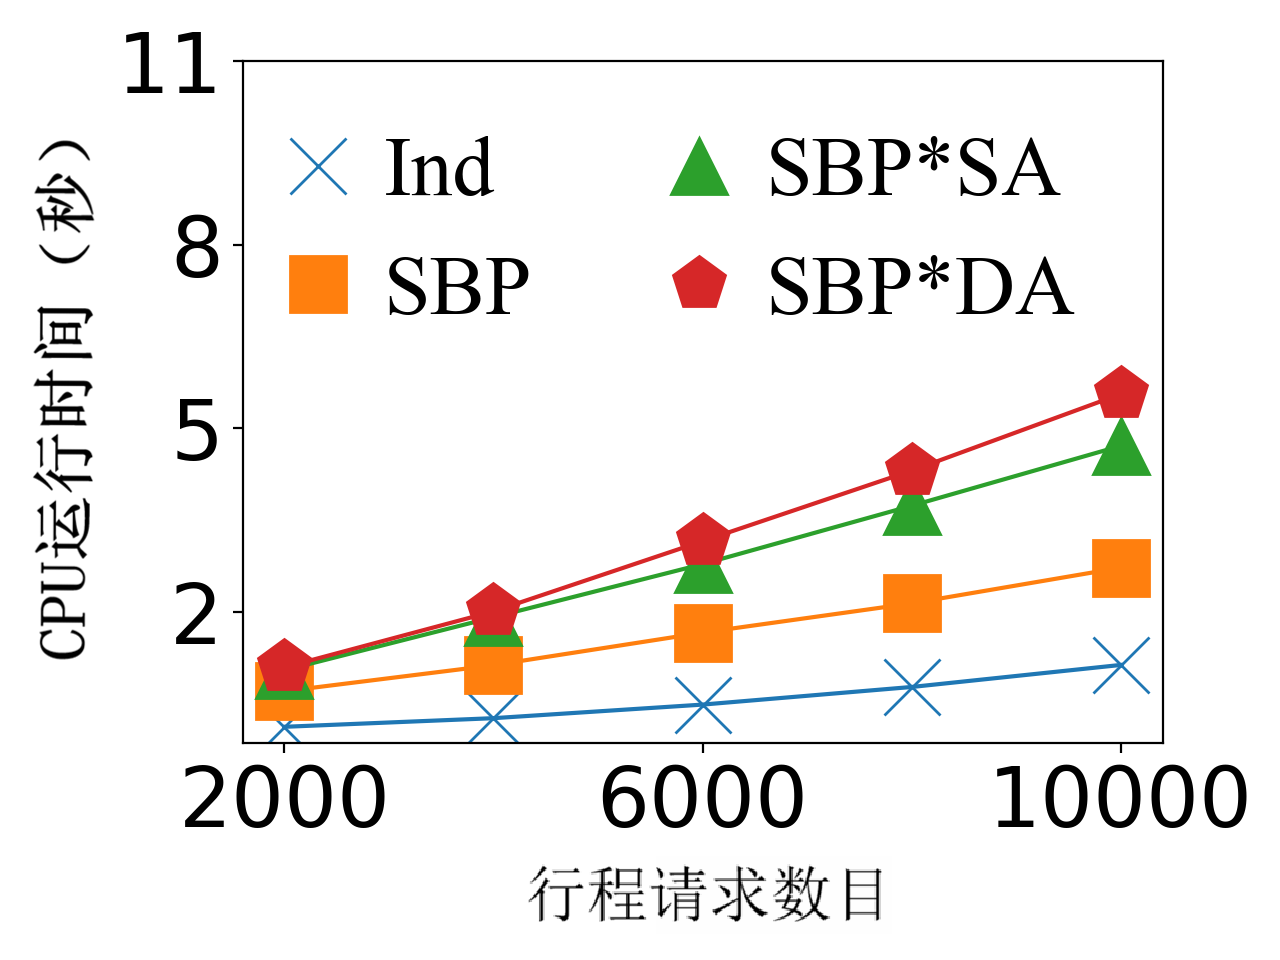
\includegraphics[width=0.4\linewidth]{fig/section3/fig1_NYC_time.png}
            \label{fig1:a}
        }%
        \hfill
        \subfloat[NY]{
        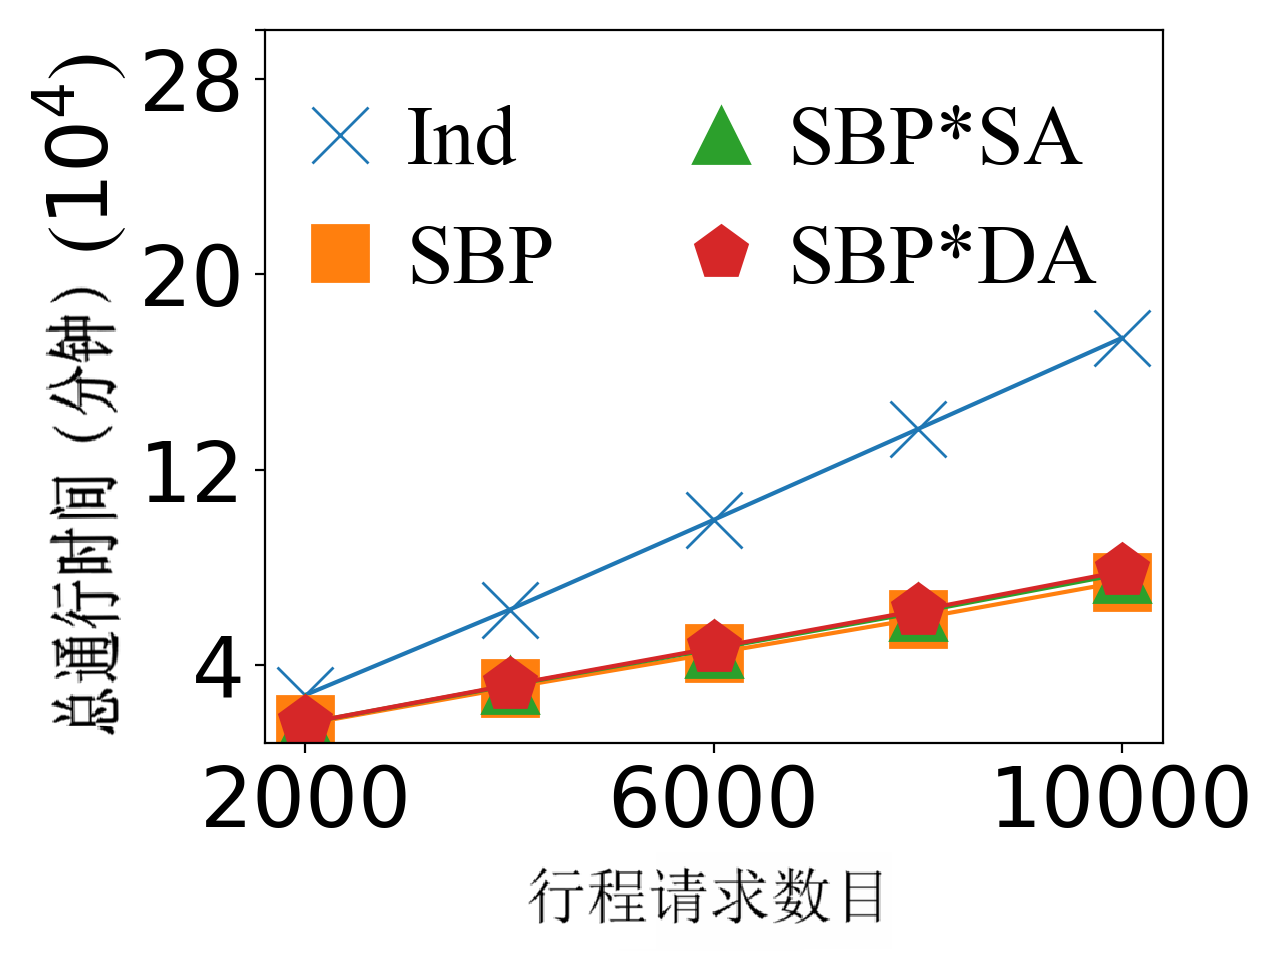
\includegraphics[width=0.4\linewidth]{fig/section3/fig1_NYC_cost.png}
            \label{fig1:b}
        }%
        \\
        \subfloat[TG]{
        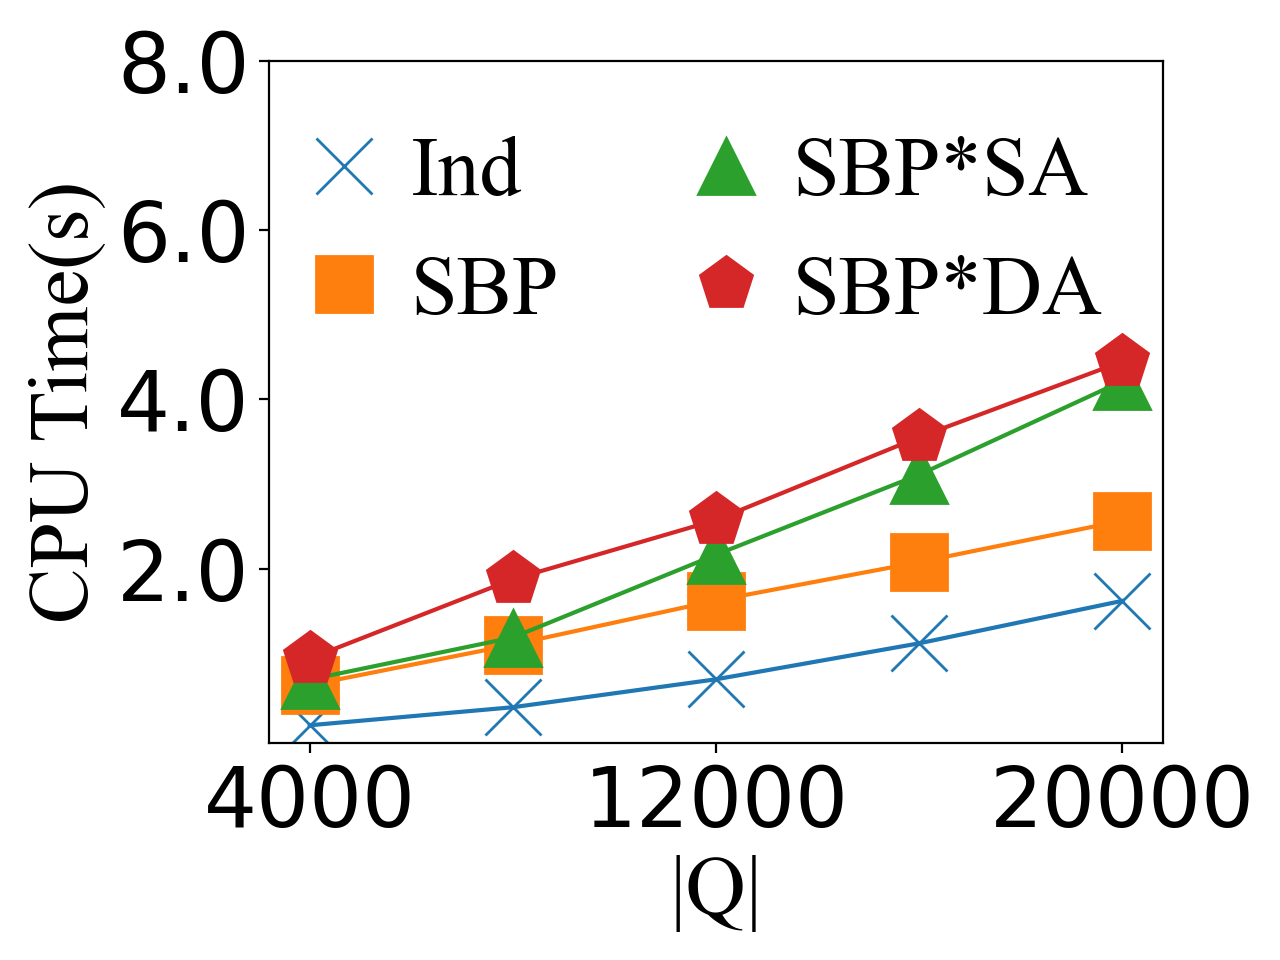
\includegraphics[width=0.4\linewidth]{fig/section3/fig1_TGC_time.png}
            \label{fig1:c}
        }%
        \hfill
        \subfloat[TG]{
        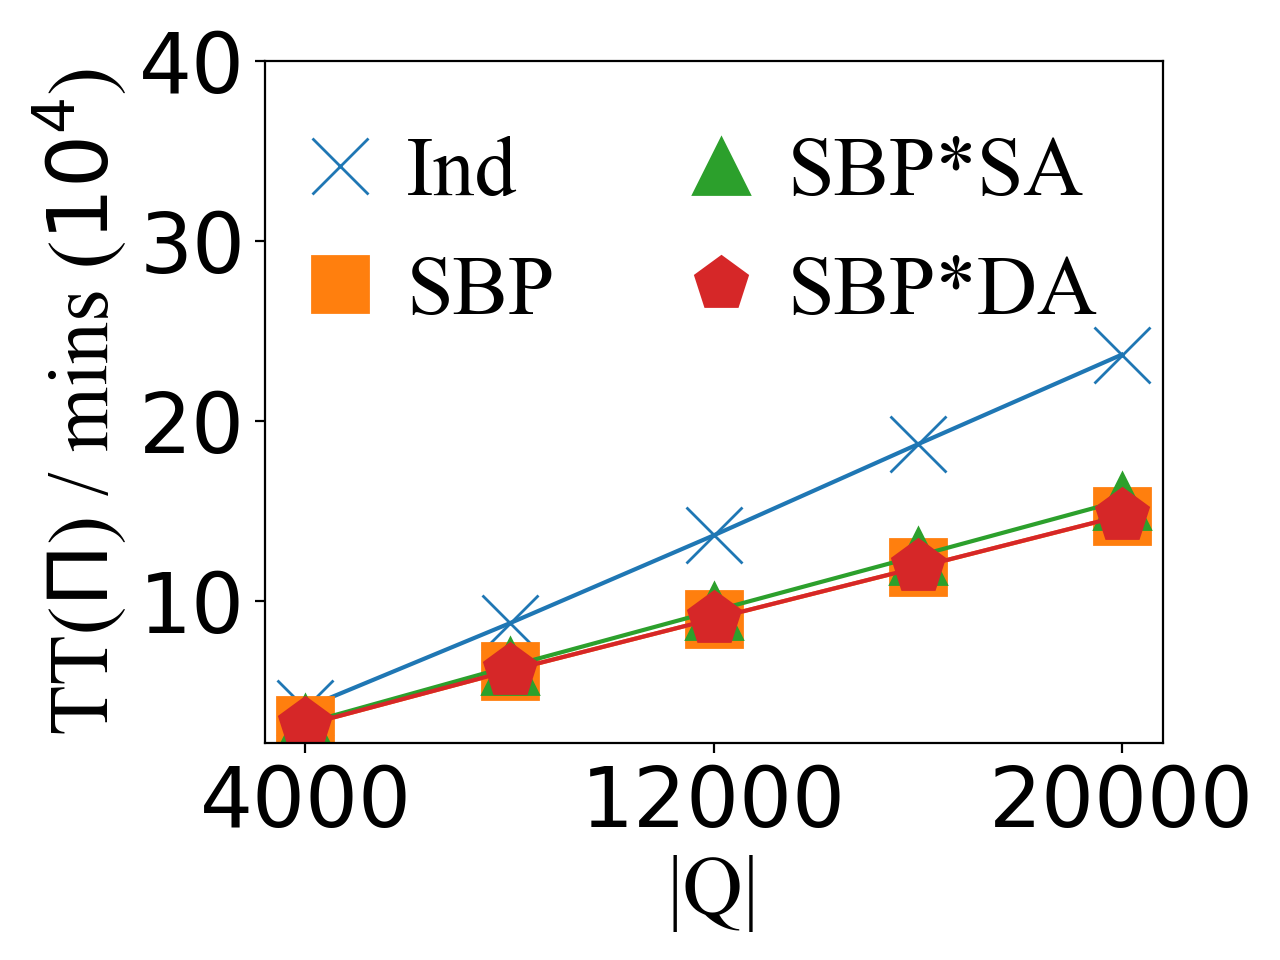
\includegraphics[width=0.4\linewidth]{fig/section3/fig1_TGC_cost.png}
            \label{fig1:d}
        }%
        \caption{行程请求数目$|Q|$的影响}
        \label{fig1}
    \end{figure*}


\begin{figure*}[h]
% Figure 2 effect Of Query arrival rate
\centering
        \subfloat[CPU time]{
            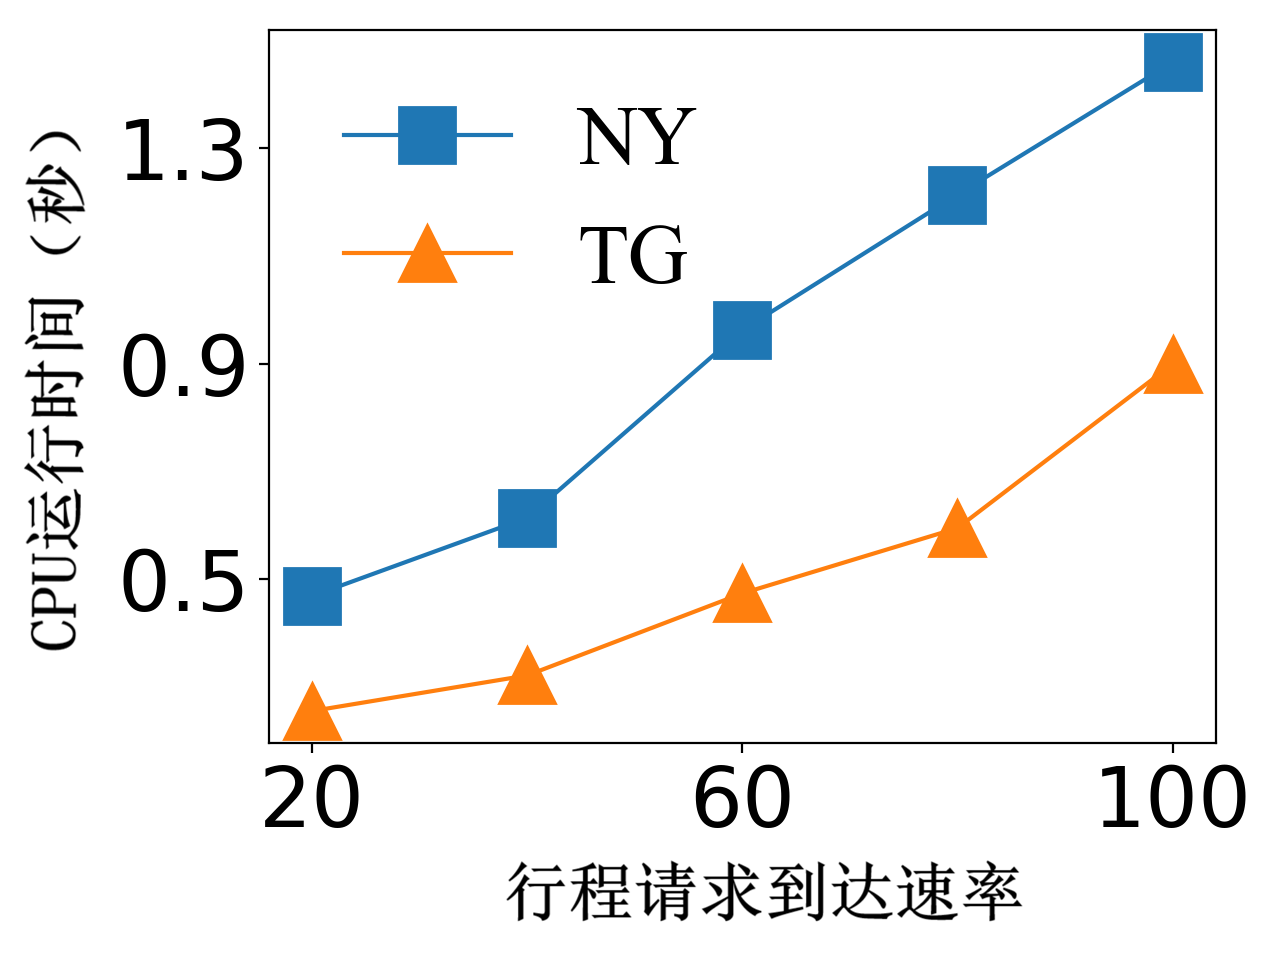
\includegraphics[width=0.4\linewidth]{fig/section3/fig2_time.png}
            \label{fig2:a}
        }% 
        \hfill
        \subfloat[Travel time]{
        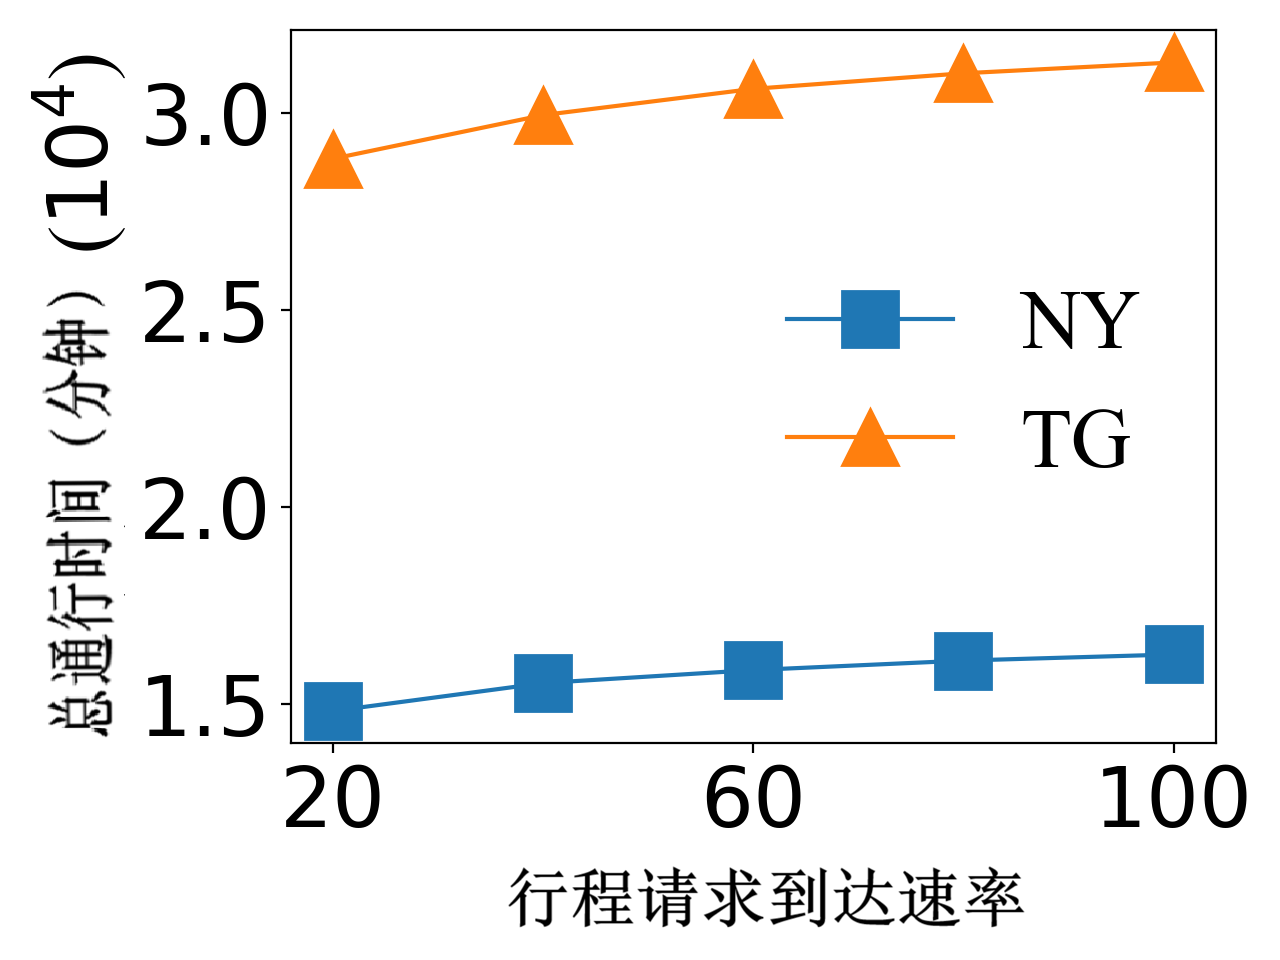
\includegraphics[width=0.4\linewidth]{fig/section3/fig2_cost.png}
            \label{fig2:b}
        }%
        \caption{行程请求到达速率的影响}
        \label{fig2}
\end{figure*}

\begin{figure*}[htbp]
% Figure 3 effect Of Refining Interval
\centering
        \subfloat[CPU time]{
            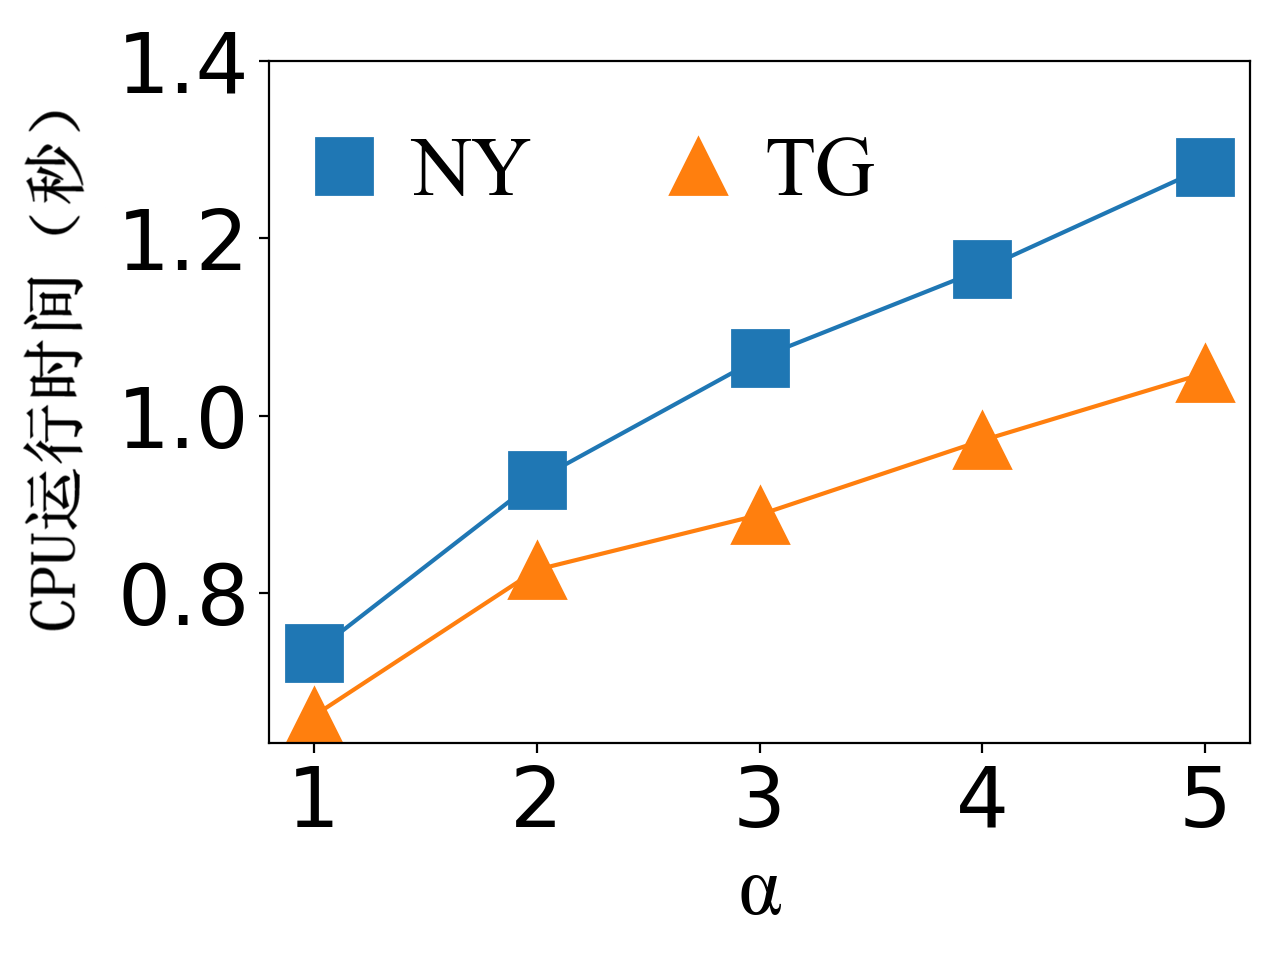
\includegraphics[width=0.4\linewidth]{fig/section3/fig3_alpha_time.png}
            \label{fig3:a}
        }%
        \hfill
        \subfloat[Travel time]{
        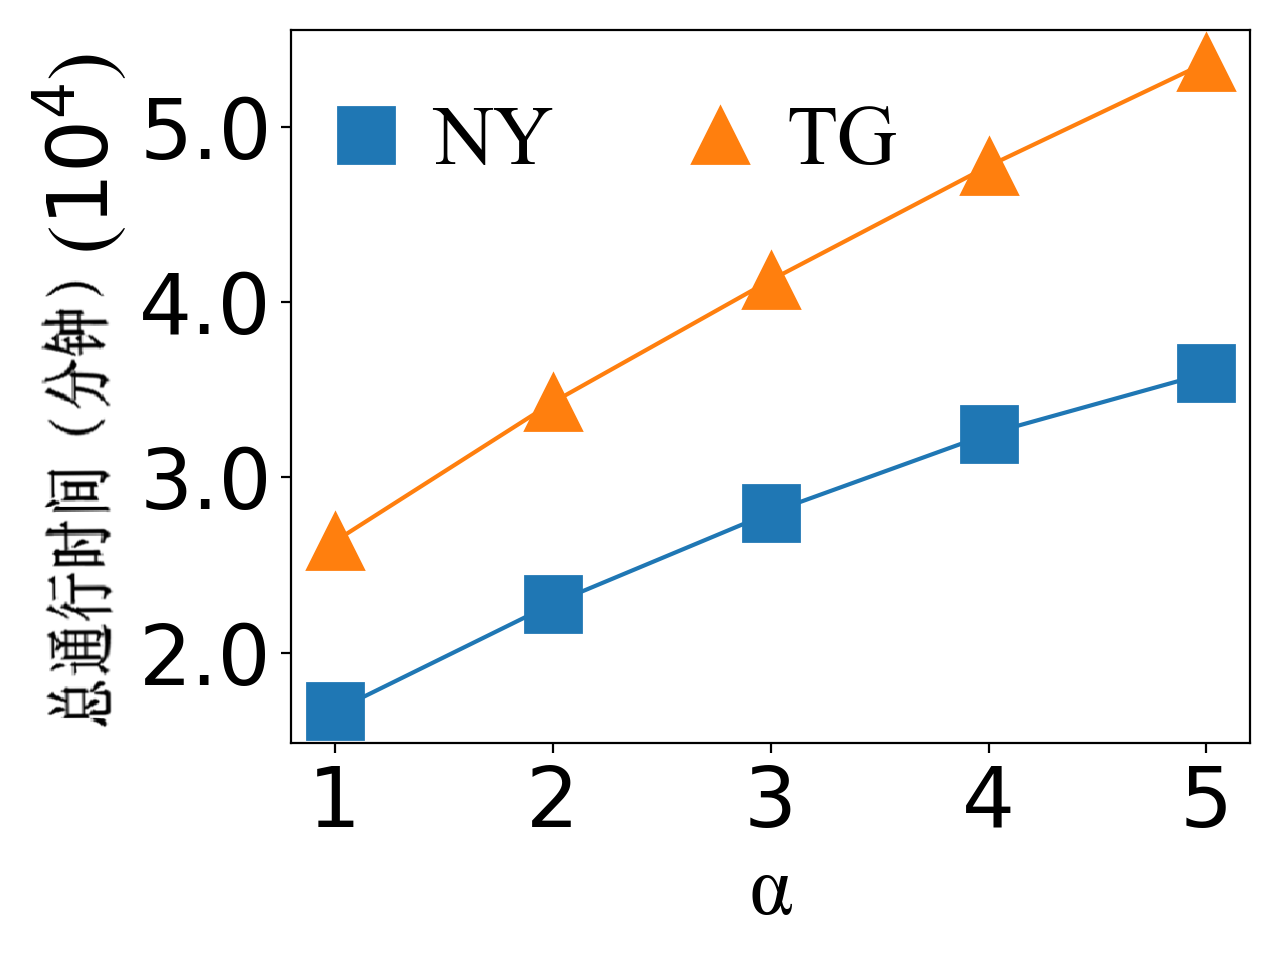
\includegraphics[width=0.4\linewidth]{fig/section3/fig3_alpha_cost.png}
            \label{fig3:b}
        }%
        \\
        \subfloat[CPU time]{
        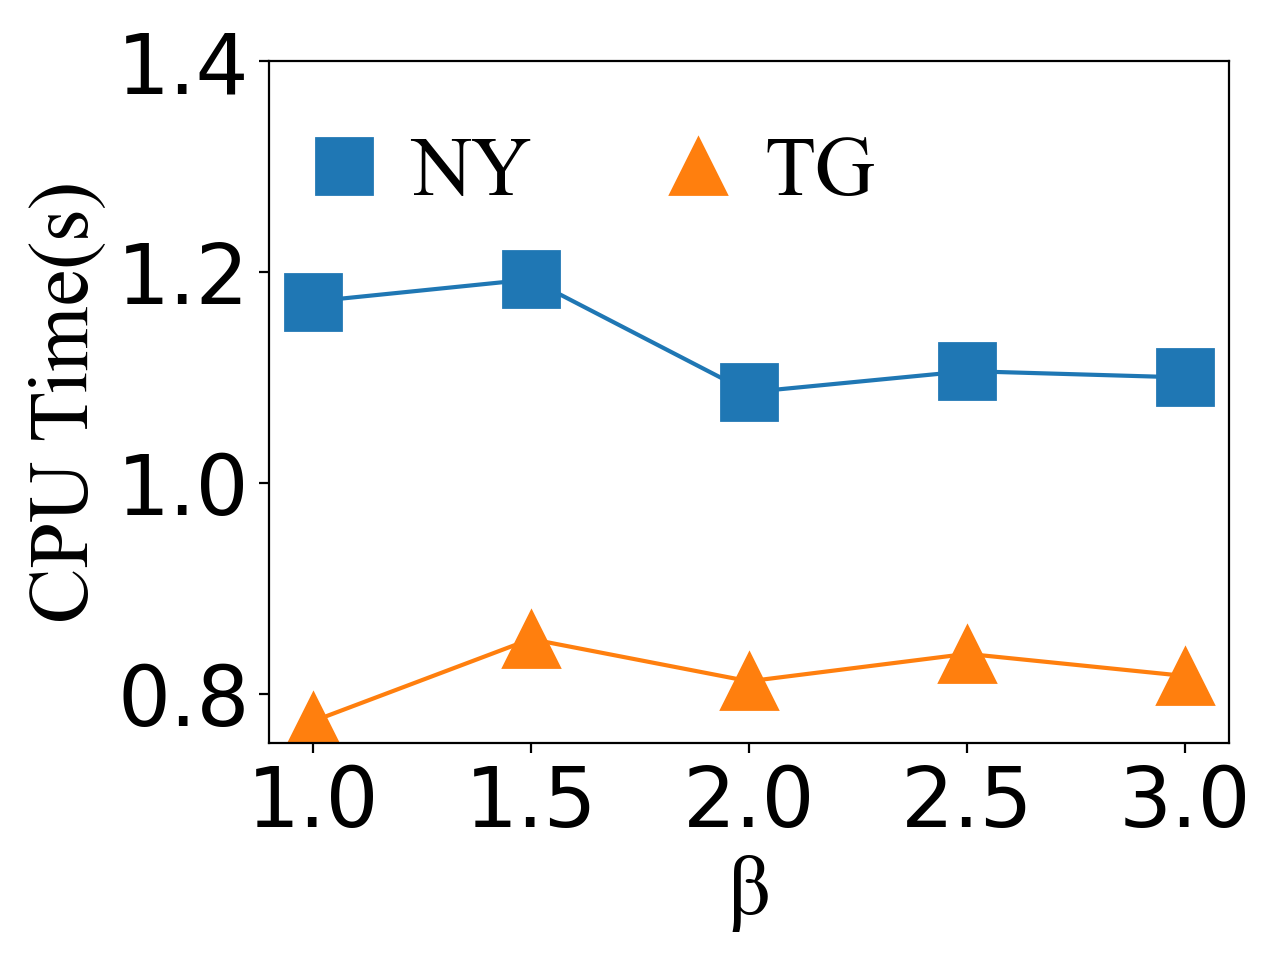
\includegraphics[width=0.4\linewidth]{fig/section3/fig3_beta_time.png}
            \label{fig3:c}
        }%
        \hfill
        \subfloat[Travel time]{
        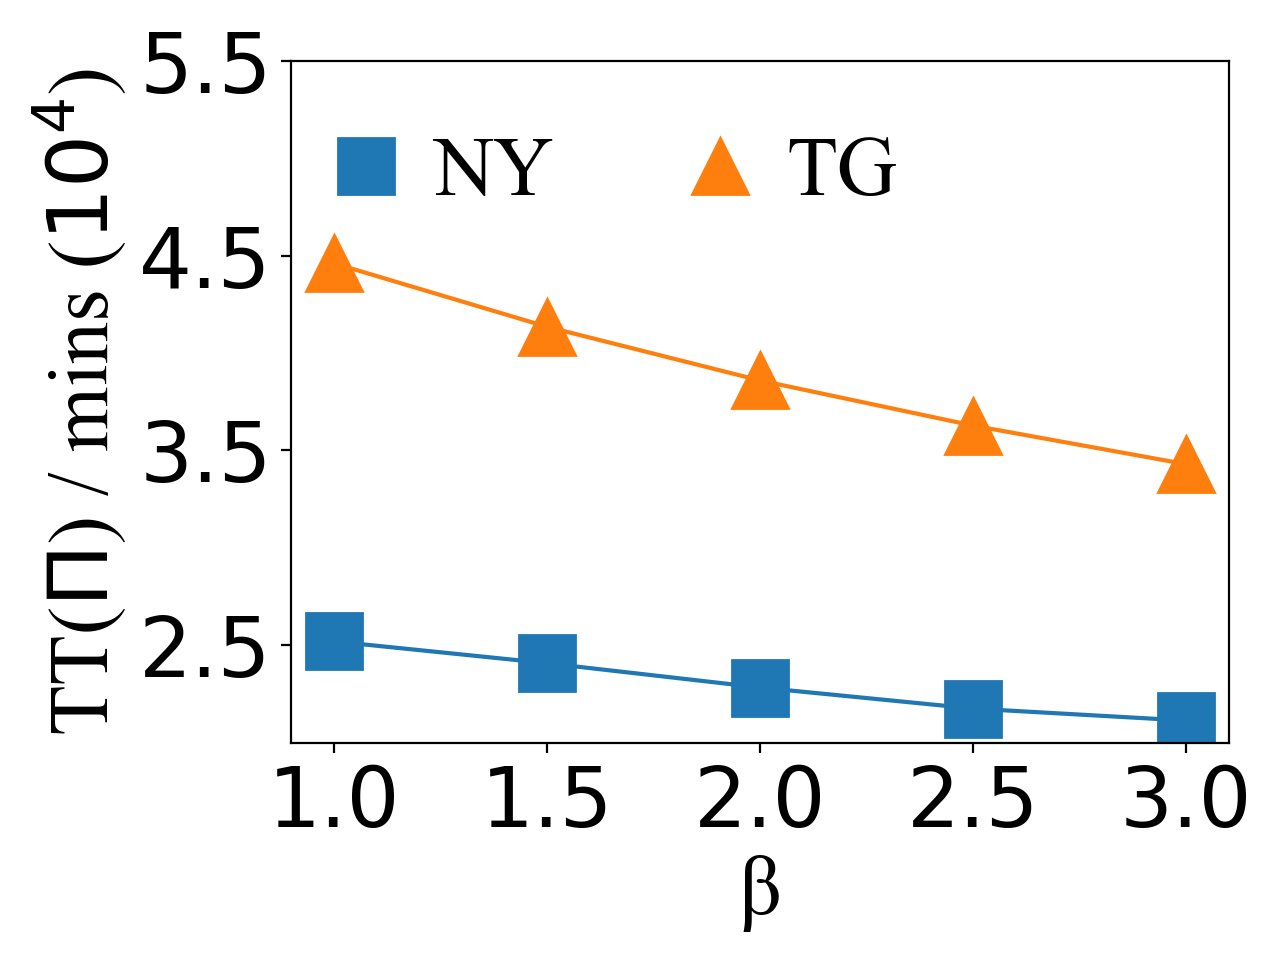
\includegraphics[width=0.4\linewidth]{fig/section3/fig3_beta_cost.png}
            \label{fig3:d}
        }%
        \caption{参数 $\alpha$ \& $\beta$的影响}
        \label{fig3}
    \end{figure*}
% Figure 4 effect Of T
\begin{figure*}[htbp]
    \centering
        \subfloat[CPU time]{
            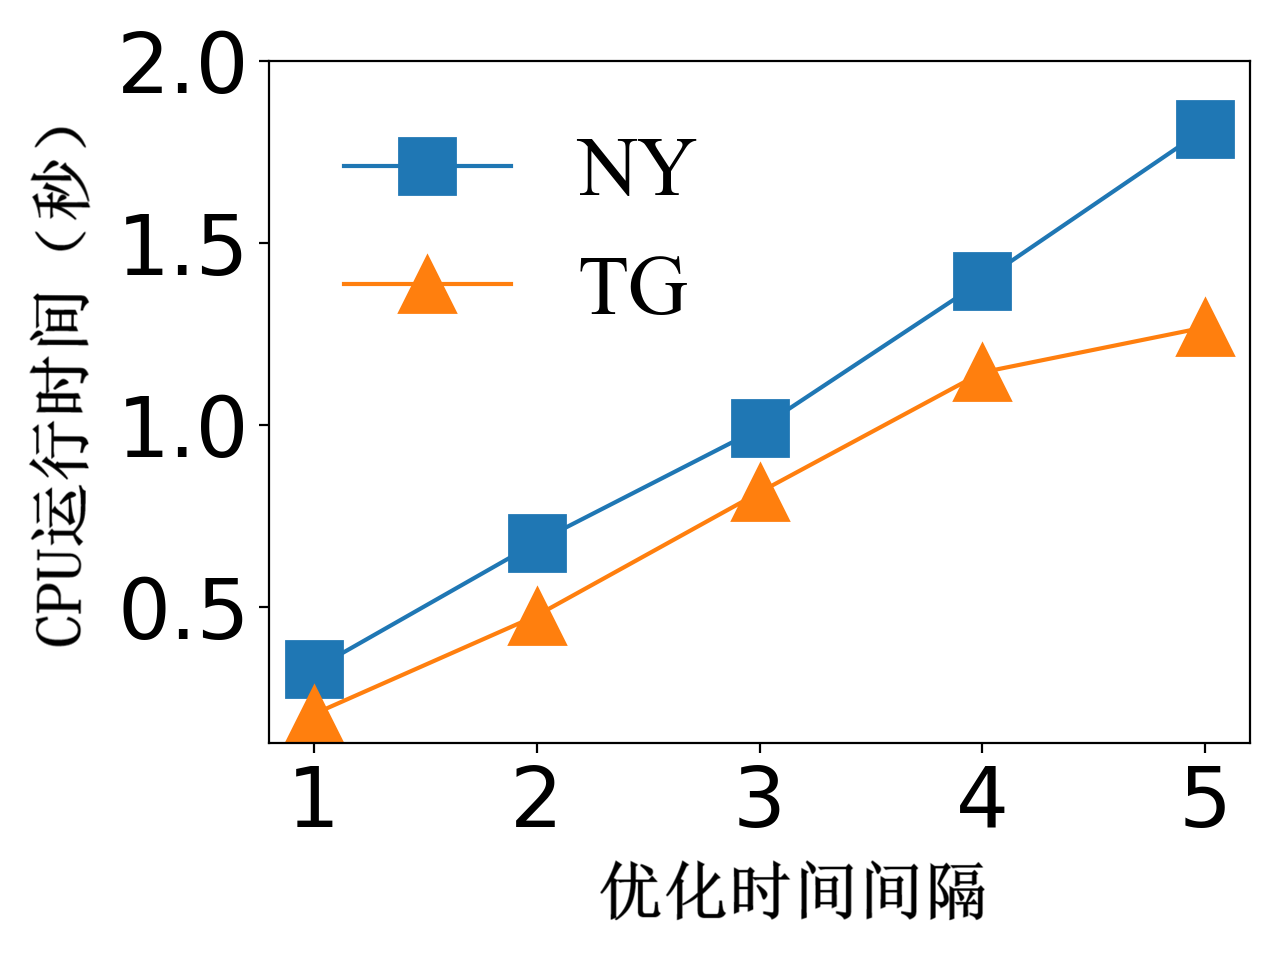
\includegraphics[width=0.4\linewidth]{fig/section3/fig4_time.png}
            \label{fig4:a}
        }% 
        \hfill
        \subfloat[Travel time]{
        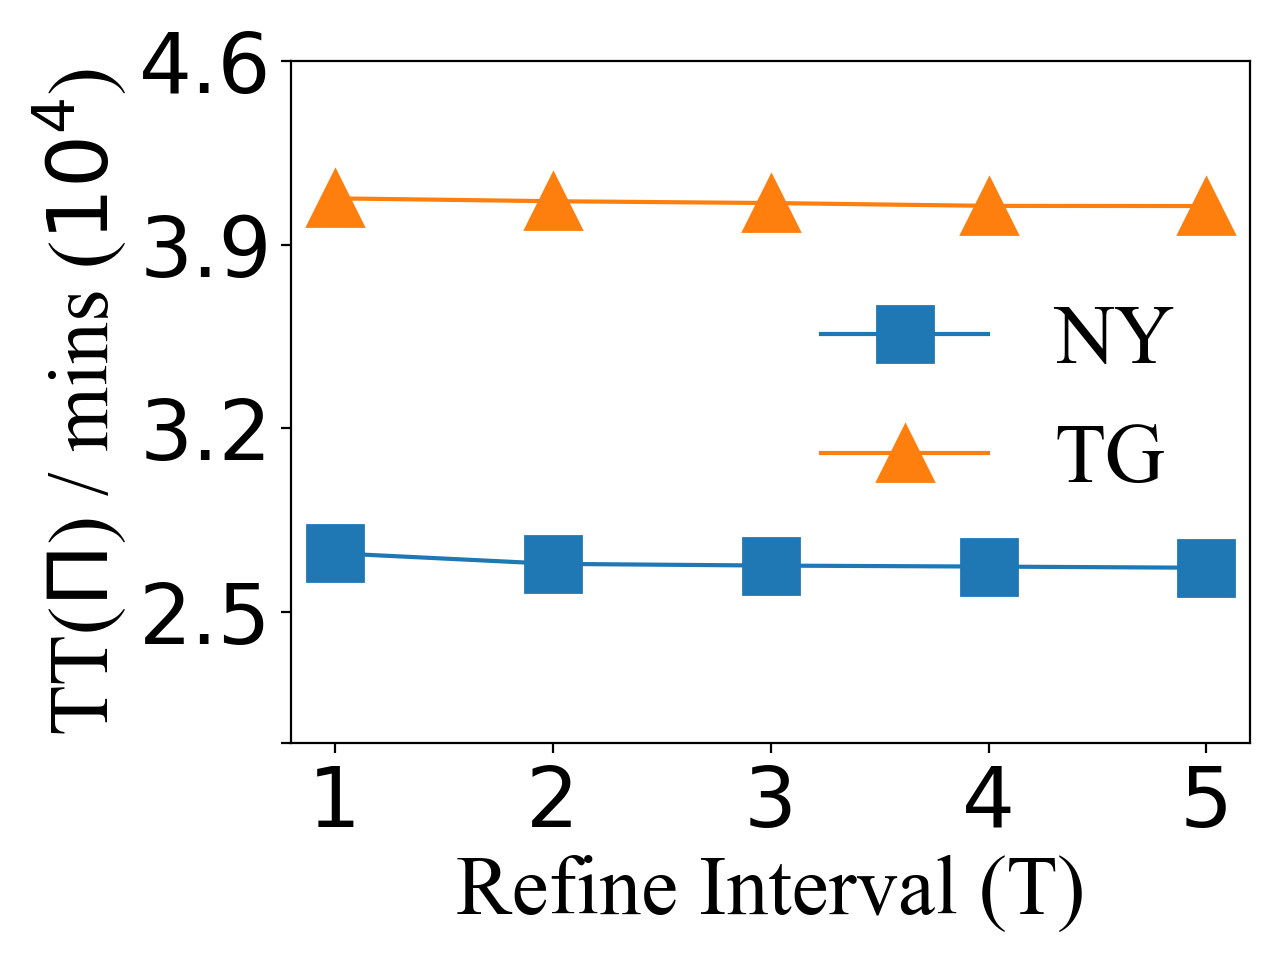
\includegraphics[width=0.4\linewidth]{fig/section3/fig4_cost.png}
            \label{fig4:b}
        }%
        \caption{批优化时间间隔T的影响}
        \label{fig4}
\end{figure*}

首先，在默认的参数设定下，我们调查了提出的算法在不同行程请求数目$|Q| $下的算法表现。直觉上，行程请求数目$ |Q| $越大，所有行程路线的总的通行时间会增加。此外，一个更大的$ |Q|$也会造成更大的计算消耗，CPU运行时间也会增加。图\ref{fig1}展示了我们提出的算法在TG路网和NY路网上的表现。意料之中的，随着行程请求数$|Q|$的增加，所有算法所需要的CPU时间都增加了。在这些算法中，基于个人的Ind算法需要的CPU时间最小，因为它是一次规划的，没有经过我们所提出的批优化处理这一过程。我们也同时发现Ind算法产生的全局路线组合中所有路线总的通行时间$TT(\Pi)$比其他算法更大，特别是在行程请求数目较大的情况下 (e.g., 当在NY路网中$|Q|=10,000$和在TG路网中 NY $|Q|=20,000$时, 和Ind算法比较，我们的SBP
算法能够减少超过40\%的通行时间).

和SBP算法相比，SBP*SA和SBP*DA表现较差。因为它们会在优化过程中进行较多次数的交换操作，这是非常耗时的。具体来说，SBP*SA没有考虑到已经规划的路线也会对路段交通增加额外的车流量，因此它在初始化路线搜索阶段进行的交通预测是不可靠的。对于SBP*DA算法，它以一个行程出发时刻的交通状态快照进行路径规划。因此，SBP*SA算法和SBP*DA算法所指定的初始化路线往往是低质量的，需要在批优化过程中采取大量的交换操作来对这些低质量的初始路线进行调整，从而产生了更多的计算消耗去提高结果质量。从图\ref{fig1:b}和图\ref{fig1:d}我们也观察到这三种算法产生的全局路线组合的所有路线的总的通行时间是非常接近的，而且我们的SBP算法总能产生较小的通行时间$TT(\Pi)$。这些实验结果证实了通过采用自感知的思想和考虑到网络动态性，我们的初始路线搜索能够有效地产生高质量的
处理路线，这样的初始路线可以减少后续优化处理过程中的交换操作次数。





\subsubsection{行程请求到达速率对算法效果的影响}
图\ref{fig2}展示了当行程请求到达速率发生改变时SBP算法的算法表现。行程请求到达速率越大，说明单位时间会有更多的车流涌入到路网的各个路段上。在这种情况下，每个路段车流量的增幅会更加明显。从而，每个路段上会产生更多的额外车流量。在图\ref{fig2}，观察CPU时间和总的通行时间$TT(\Pi)$，不管是在NY路网还是在TG路网上，我们都可以发现它们有明显的增长趋势。$TT(\Pi)$增长是因为随着车流量增加，每个路段的通行时间也相应增加了。在TG路网上，所有的行程规划的路线的总的通行时间远远大于在NY路网上的，这是因为在我们的默认设定中，TG路网会有更多数目的行程请求产生。




\subsubsection{通行时间函数各参数对算法效果的影响}
图\ref{fig3}展示了当我们变化通行时间函数中的参数$\alpha$和 $\beta$ (cf. 式 \ref{eq:tf})时SBP算法的算法表现。直觉上，$\alpha$越大或者$\beta$越小，各路段通行时间会增大，从而可能会加剧交通拥堵。在图\ref{fig3:a}中，当$\alpha$从1变化到5时，CPU时间和所有行程总的通行时间都有增加的趋势。相反的，当$\beta$从1变化到3时，总的通行时间具有下降的趋势。值得注意的是，当我们变化$\beta$时，CPU时间没有特别明显的变化趋势，这是因为CPU时间即我们所需要的计算消耗并不是和 $\beta$的值直接相关的。

\subsubsection{优化时间间隔对算法表现的影响}
图\ref{fig4}展示了当优化时间间隔$T$变化时SBP算法的表现。$T$越大代表着每个请求的等待时间增加了，但是规划的结果会更趋于最优，这是因为有更多的正在规划的路线被考虑到了对未来的交通状态影响中去了。在这种情况下，我们通过交换操作大大减少所有行程总的通行时间$TT(\Pi)$。在图\ref{fig4:a}，CPU时间随着$T$的增加而增加，这是因为我们在一次优化过程中需要处理更多的行程请求。在图\ref{fig4:b}中，我们可以发现$TT(\Pi)$有一个轻微的减小趋势。这些结果说明了一个合适的优化时间间隔能够通过重新利用已经规划的初始路线来更准确地未来的交通状态，从而避免交通拥堵。

\begin{figure}[h]
% 	Figure 1 effect Of Query Count
        \centering
        \subfloat[]{
            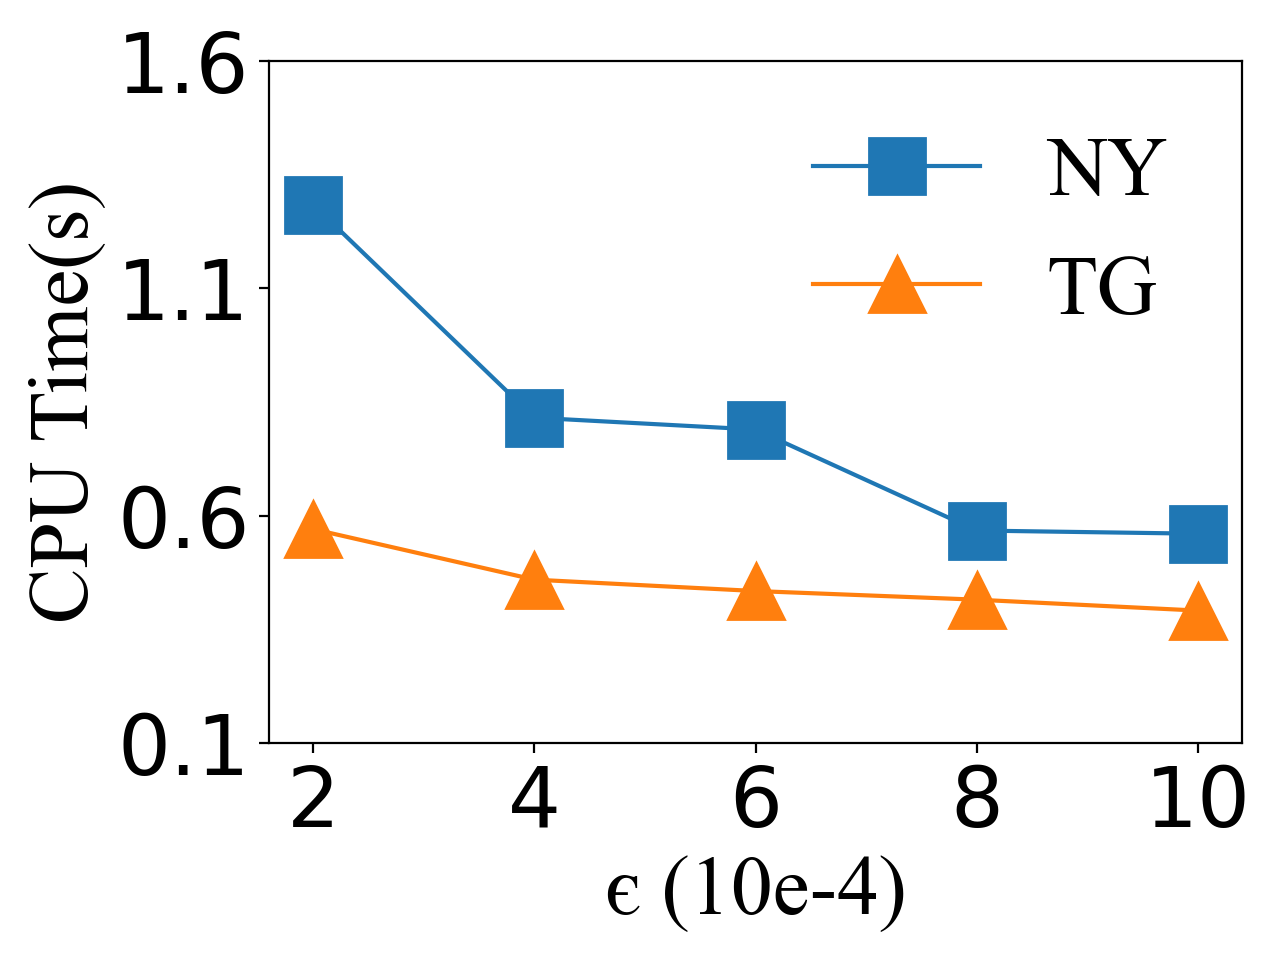
\includegraphics[width=0.33\linewidth]{fig/section3/fig5_time.png}
            \label{fig5:a}
        }%
        \subfloat[]{
            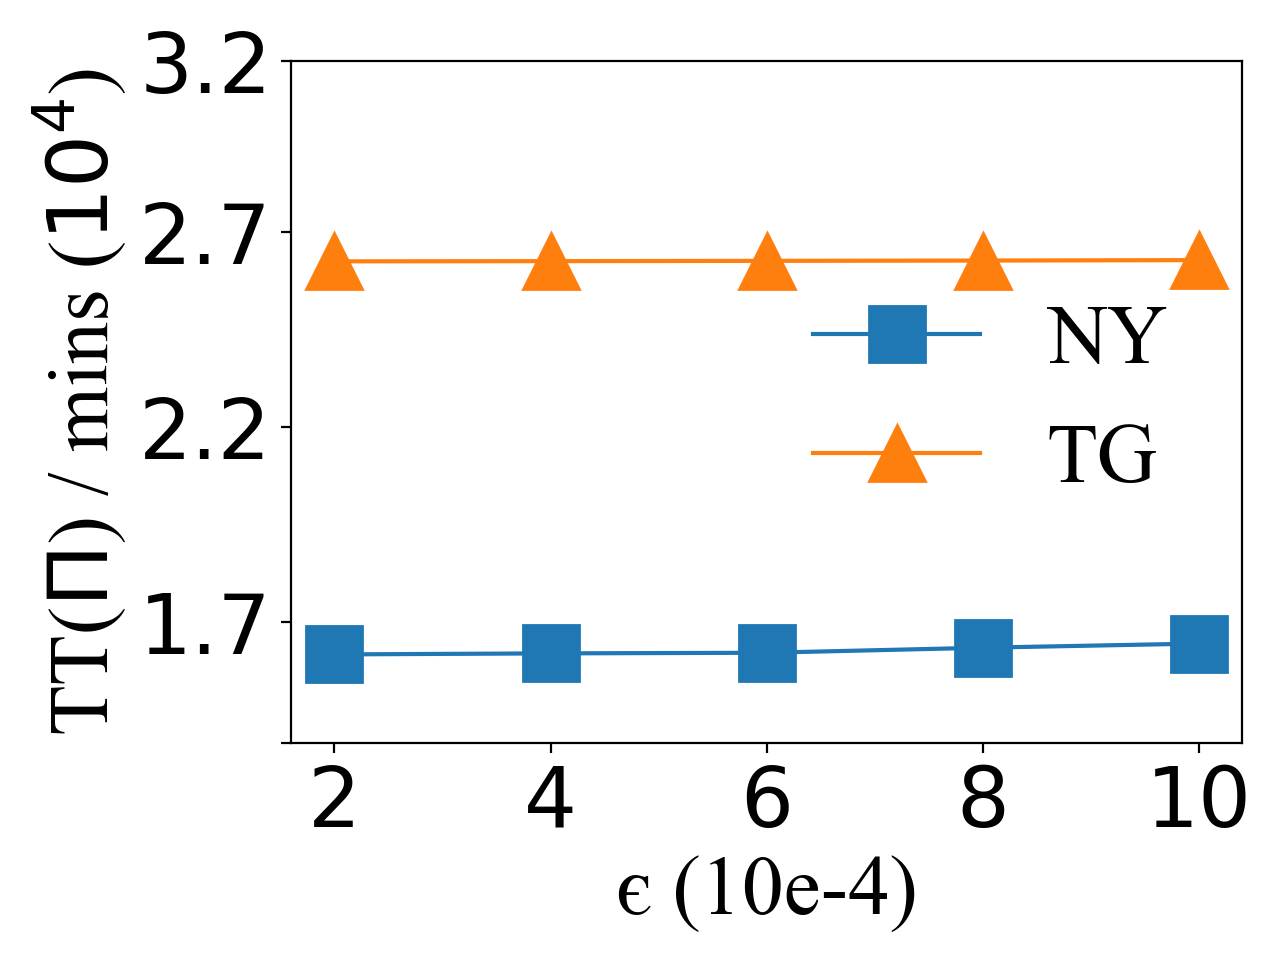
\includegraphics[width=0.33\linewidth]{fig/section3/fig5_cost.png}
            \label{fig5:b}
        }%
        \subfloat[]{
        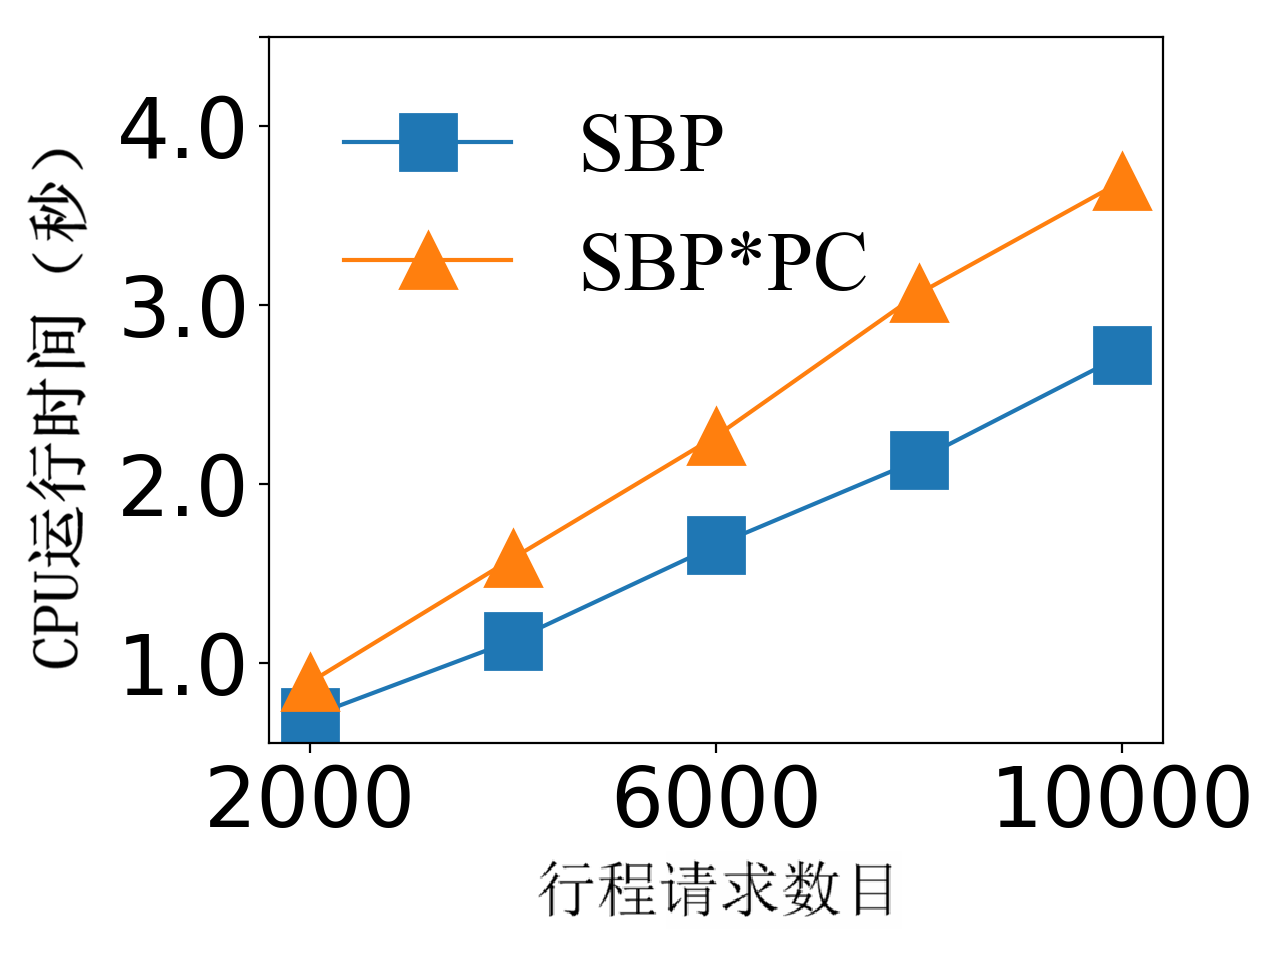
\includegraphics[width=0.33\linewidth]{fig/section3/fig6_NY.png}
            \label{fig5:c}
        }% 
        \caption{参数$\epsilon$和预检查策略的影响 \subref{fig5:a} CPU运行时间；\subref{fig5:b} 通行时间；\subref{fig5:a} 预先检查策略的影响评估 }
        \label{fig5}
\end{figure}

\subsubsection{参数$\epsilon$和预检查策略对算法表现的影响}
我们研究了当参数$\epsilon$从0.0002变化到 0.001时的SBP算法表现。我们知道在优化处理过程中，总的有效交换操作的次数是和参数$\epsilon$的值成反比的 (cf. 算法 \ref{alg:alg3})。$\epsilon$越大，意味着有效操作的门槛越高，有效操作的次数越少，因此CPU时间也会随之减少。然而，一个更大的$\epsilon$也会产生具有更大通行时间的全局路线组合$\Pi$。在图\ref{fig5:a}中，当参数$\epsilon$从0.0002变化到 0.001时，CPU时间有一个减少的趋势。
相反的，所有行程总的通行时间有一个轻微的增加的趋势。当$\epsilon$从0.0002 变化到0.0004时，所需要的CPU时间降幅最大 (e.g., 在NY路网和TG路网中，需要的CPU时间减少幅度分别超过了 36\% 和 19\%).  我们也发现对于$\epsilon$值的选取，0.001是非常合适的，从图中我们可以看出当$\epsilon$为0.001时，算法的综合表现是最好的。以上实验结果说明通过利用一个合适的参数$\epsilon$，SBP算法的表现能够得到较大的提升。 我们用"SBP*PC"来表示没有应用预检查策略的SBP算法，在图\ref{fig5:c}中，我们观察到SBP算法所需要的CPU运行时间总是比SBP*PC算法更少，这个实验结果说明了我们提出的预检查策略是能够进一步提升算法效率的。


\section{本章小结}
我们提出和调查了一个新颖的路线规划问题（CORC问题)，该问题旨在为持续的形成请求搜寻最佳的路线组合 。我们提出了一个SBP算法来高效解决CORC问题。同时，一些修剪枝技术的提出也大大提升了算法效率。对应的实验研究证实了我们提出的算法能够有效地解决该问题，也证实了我们提出的剪枝技术有够有助于避免不必要的计算。
